\newpage
\section{Giới Thiệu}
\subsection{Lý do chọn đề tài}
Trong những năm gần đây, thương mại điện tử ngày càng phát triển và trở thành một phần quan trọng trong hoạt động kinh doanh. Cùng với sự phát triển đó, các nền tảng thương mại điện tử tạo ra một lượng lớn dữ liệu liên quan đến khách hàng, đơn hàng, sản phẩm, người bán, thanh toán và vận chuyển. Nguồn dữ liệu này không chỉ phản ánh tình hình kinh doanh mà còn chứa nhiều thông tin có giá trị cho việc đánh giá và đưa ra các quyết định phù hợp.

Tuy nhiên, khi dữ liệu được lưu trữ ở nhiều nguồn và dưới nhiều dạng khác nhau, việc tổng hợp và khai thác trực tiếp trên hệ thống giao dịch gặp nhiều khó khăn. Do đó, việc xây dựng một kho dữ liệu tập trung giúp tổ chức, lưu trữ và quản lý dữ liệu một cách có hệ thống, đồng thời tạo nền tảng thuận lợi cho quá trình phân tích và khai thác thông tin.

Xuất phát từ những lý do trên, nhóm lựa chọn đề tài \textbf{“Xây dựng kho dữ liệu và phân tích hiệu quả kinh doanh trên nền tảng thương mại điện tử”} dựa trên bộ dữ liệu Olist. Thông qua đề tài, nhóm hướng đến việc xây dựng kho dữ liệu phục vụ phân tích các khía cạnh như doanh thu, đơn hàng, sản phẩm, khách hàng và người bán theo nhiều chiều dữ liệu khác nhau. Qua đó, đề tài giúp vận dụng các kiến thức về \textbf{Kho dữ liệu và OLAP} vào một bài toán thực tế, đồng thời tạo ra cơ sở để tổng hợp và khai thác các thông tin phục vụ đánh giá hiệu quả hoạt động kinh doanh trên nền tảng thương mại điện tử.
\subsection{Giới thiệu về dataset}
\subsubsection{Tổng quan dataset}
Tập dữ liệu thương mại điện tử Olist (Brazil) dạng cơ sở dữ liệu quan hệ SQLite, lưu trữ toàn bộ chu trình kinh doanh trực tuyến thực tế: từ đơn hàng, thông tin khách hàng, người bán, danh mục sản phẩm, phương thức thanh toán, vận chuyển cho đến đánh giá (reviews).
\subsubsection{Mô tả quy mô và thời gian thu thập}
\textbf{Nguồn dữ liệu:} Bộ dữ liệu được công bố công khai trên Kaggle: \href{https://www.kaggle.com/datasets/terencicp/e-commerce-dataset-by-olist-as-an-sqlite-database}{E-commerce dataset by Olist as an SQLite database}.

\textbf{Thời gian thu thập:} Từ tháng 09/2016 đến tháng 10/2018 (đơn hàng sớm nhất ngày 04/09/2016, đơn hàng muộn nhất ngày 17/10/2018).

\textbf{Cấu trúc:} Gồm \textbf{11 bảng quan hệ} (\texttt{orders}, \texttt{customers}, \texttt{order\_items}, \texttt{order\_payments}, \texttt{order\_reviews}, \texttt{products}, \texttt{product\_category\_name\_translation}, \texttt{sellers}, \texttt{geolocation}, \texttt{leads\_qualified}, \texttt{leads\_closed}) liên kết với nhau qua các khóa chính và khóa ngoại.

\textbf{Số dòng:} Tổng cộng \textbf{1.559.764 dòng} trên toàn bộ 11 bảng, trong đó có \textbf{99.441 đơn hàng} và \textbf{112.650 dòng chi tiết đơn hàng}; riêng bảng tọa độ \texttt{geolocation} chiếm 1.000.163 dòng.

\textbf{Số cột:} Tổng cộng \textbf{70 cột thuộc tính} phân bổ trên 11 bảng (mỗi bảng từ 2 đến 14 cột).

Cấu trúc ban đầu của bộ dữ liệu cùng quan hệ giữa các bảng được thể hiện trong Hình~\ref{fig:c1_csdl_goc}.

\begin{figure}[H]
    \centering
    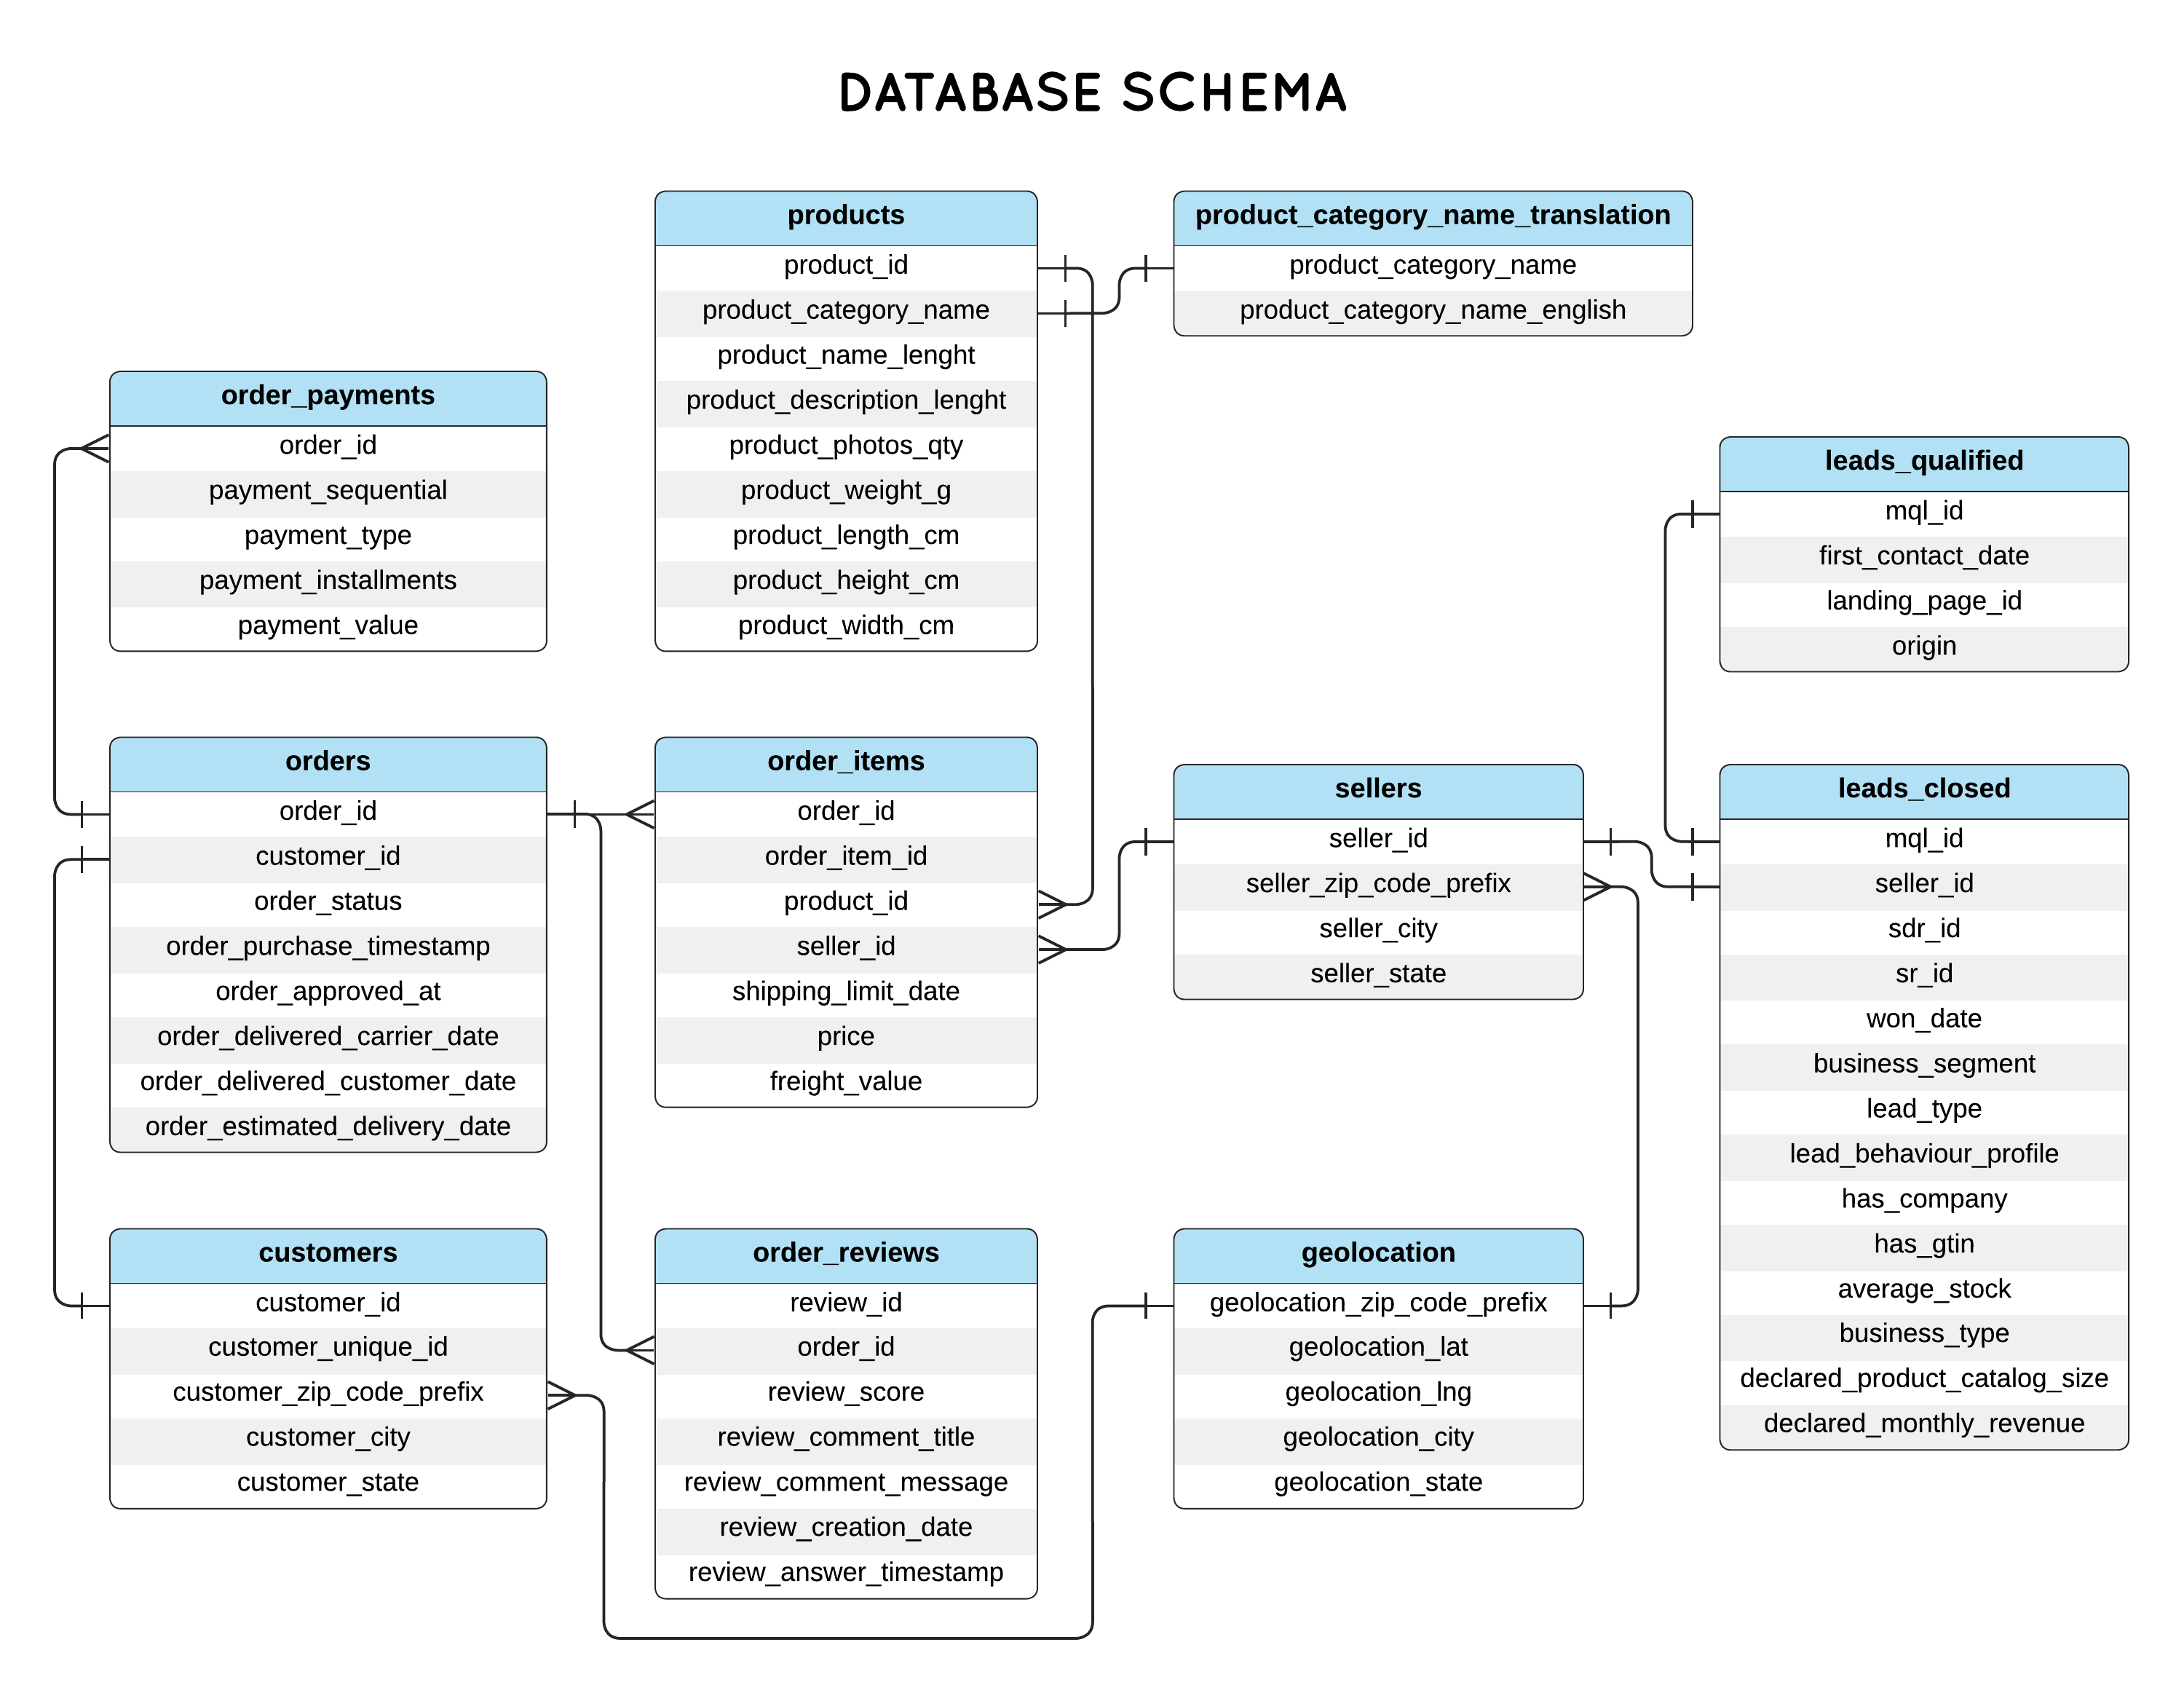
\includegraphics[width=\textwidth]{img_c1/c1_fig01_luoc_do_csdl_goc.png}
    \caption{Lược đồ quan hệ của bộ dữ liệu Olist gốc gồm 11 bảng}
    \label{fig:c1_csdl_goc}
\end{figure}

\subsection{Quy trình tiền xử lý dữ liệu}\label{subsec:tienxuly}

Toàn bộ quy trình tiền xử lý dữ liệu được thực hiện bằng Python (sử dụng hai thư viện chính là \texttt{pandas} và \texttt{numpy}), xử lý dữ liệu thô từ các tệp CSV trích xuất từ cơ sở dữ liệu Olist. Mục tiêu là làm sạch dữ liệu, xử lý các dị biệt nghiệp vụ và chuẩn hóa cấu trúc để sẵn sàng nạp vào kho dữ liệu. Nội dung dưới đây trình bày chi tiết từng bước thực hiện kèm hình ảnh minh chứng từ kết quả chạy thực tế.

\subsubsection{Khám phá và phát hiện vấn đề dữ liệu}

Trước khi thực hiện biến đổi, tiến hành khảo sát cấu trúc thực thể, tính duy nhất của khóa chính (PK) và mối quan hệ giữa các bảng dữ liệu thô.

\paragraph{Kiểm tra số lượng dòng và khóa chính}

Thực hiện kiểm tra số lượng bản ghi và kiểm định tính duy nhất của khóa chính trên từng bảng nhằm phát hiện sớm các trường hợp trùng lặp hoặc vi phạm ràng buộc toàn vẹn.

\begin{figure}[H]
    \centering
    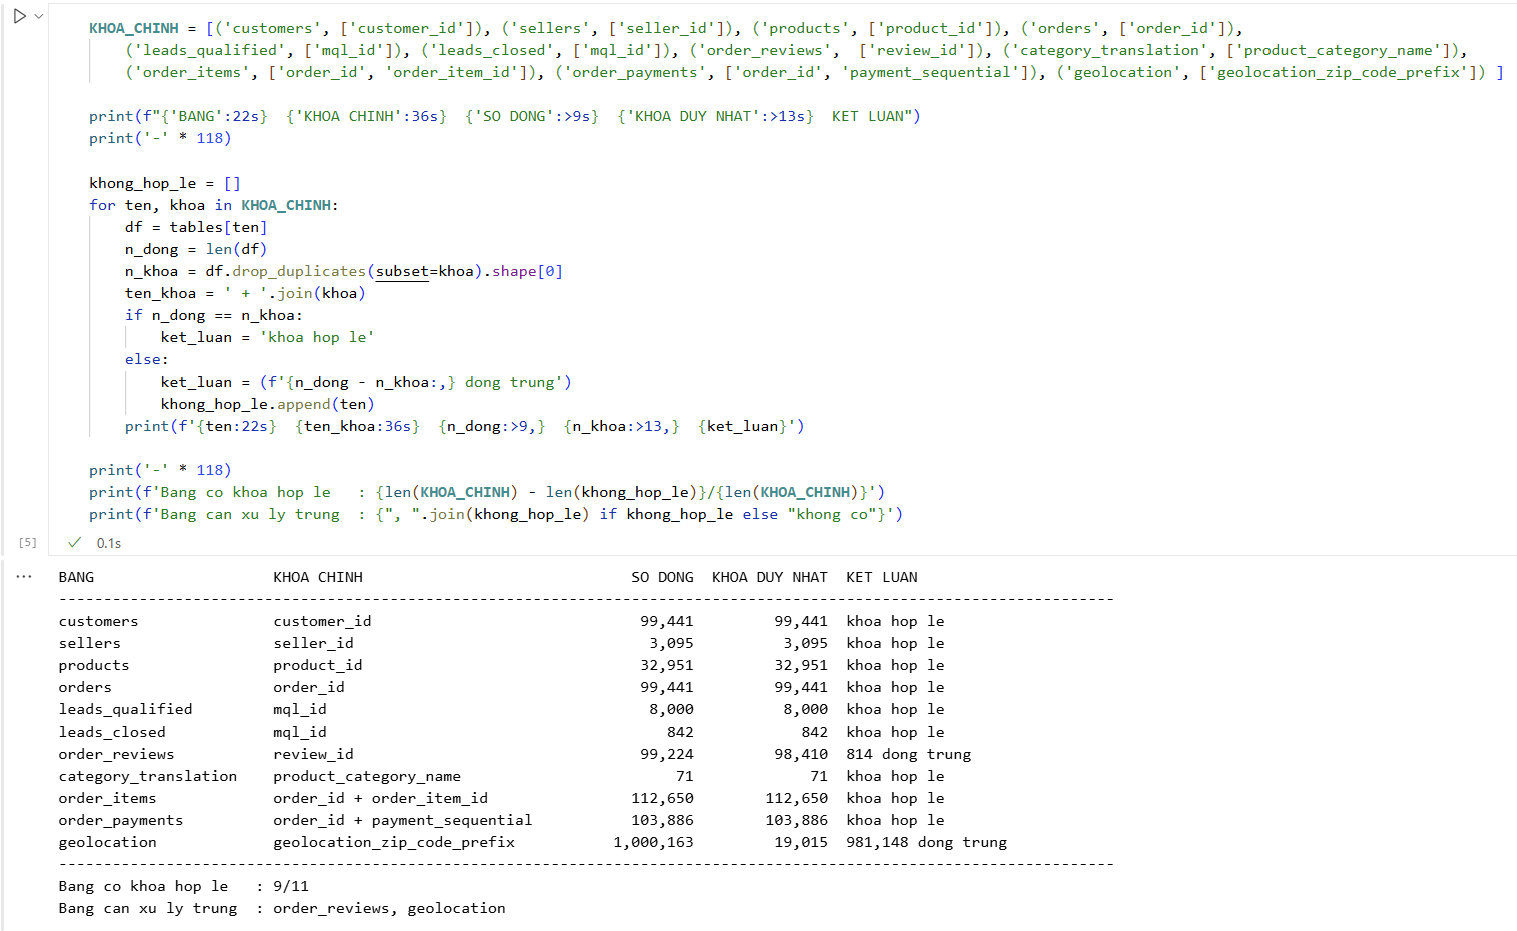
\includegraphics[width=\textwidth]{img_c1/c1_fig02_kham_pha_phat_hien_van.png}
    \caption{Kiểm tra số lượng dòng và tính hợp lệ của khóa chính trên các bảng thô}
    \label{fig:c1f02}
\end{figure}

\paragraph{Kiểm tra dữ liệu nhiều dòng trên cùng một mã đơn hàng ở bảng thanh toán và đánh giá}

Khảo sát quan hệ 1-N giữa bảng đơn hàng (\texttt{orders}) với bảng thanh toán (\texttt{order\_payments}) và bảng đánh giá (\texttt{order\_reviews}):
\begin{itemize}\setlength{\itemsep}{2pt}
  \item Ở bảng \texttt{order\_payments}, một đơn hàng có thể có nhiều dòng thanh toán do khách hàng chia nhiều đợt trả góp hoặc kết hợp nhiều hình thức thanh toán khác nhau (ví dụ: kết hợp thẻ tín dụng và voucher).
  \item Ở bảng \texttt{order\_reviews}, một đơn hàng có thể nhận nhiều dòng đánh giá do hệ thống gửi khảo sát nhắc nhở hoặc khách hàng cập nhật lại phản hồi trải nghiệm dịch vụ.
\end{itemize}

\begin{figure}[H]
    \centering
    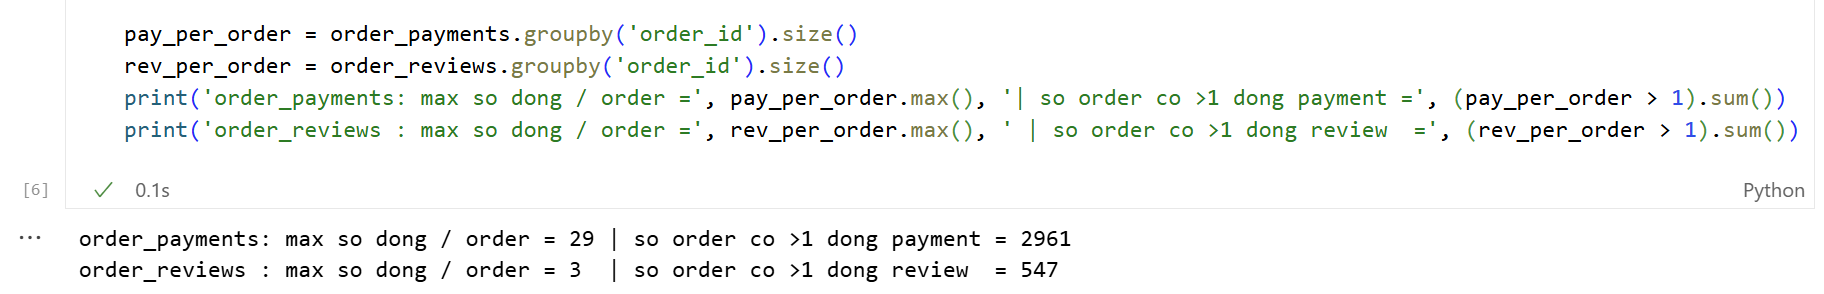
\includegraphics[width=\textwidth]{img_c1/c1_fig03_kham_pha_phat_hien_van.png}
    \caption{Kiểm tra phân bố nhiều dòng dữ liệu trên cùng một mã đơn hàng}
    \label{fig:c1f03}
\end{figure}

\subsubsection{Xử lý giá trị thiếu}

Các bước xử lý giá trị thiếu (NULL) được thực hiện trước khi xây dựng các bảng Dim và Fact, nhằm đảm bảo dữ liệu đưa vào các phép join không bị lỗi hoặc thất thoát bản ghi. Chiến lược xử lý được phân loại cụ thể theo từng nhóm tính chất trong Bảng~\ref{tab:null_rules}.

\begin{table}[htbp]
\centering
\caption{Chiến lược xử lý giá trị thiếu (NULL) theo nhóm đặc trưng}\label{tab:null_rules}
\vspace{4pt}
{\footnotesize
\begin{tabular}{@{}p{3.8cm}p{3.5cm}p{6.5cm}@{}}
\toprule
\textbf{Nhóm dữ liệu} & \textbf{Chiến lược xử lý} & \textbf{Cơ sở học thuật và nghiệp vụ} \\
\midrule
Mang tín hiệu nghiệp vụ & \textbf{Giữ nguyên} \texttt{NaN}/\texttt{NaT} & Việc điền giá trị giả sẽ làm sai lệch trạng thái thực tế của quy trình đơn hàng. \\
Text tự do, optional & \texttt{fillna('')} & Chuẩn hóa về chuỗi rỗng để tránh lỗi trong quá trình xử lý chuỗi. \\
Định danh / phân loại (FK, group-by) & \texttt{fillna} bằng placeholder & Gán nhãn quy ước (\texttt{'outros'}, \texttt{'unknown'}) để không làm mất dòng khi join hoặc gom nhóm phân tích. \\
Cột số dùng tính toán định lượng & Impute bằng \textbf{median} & Dùng trung vị (median) thay vì mean vì phân phối kích thước/trọng lượng bị lệch bởi outlier; median phản ánh đúng xu thế trung tâm hơn. \\
\bottomrule
\end{tabular}}
\end{table}

\paragraph{Rà soát tổng quan giá trị thiếu trên tất cả bảng thô}

Thực hiện rà soát tự động tỷ lệ giá trị thiếu trên toàn bộ các cột thuộc tính của 11 bảng thô.

\begin{figure}[H]
    \centering
    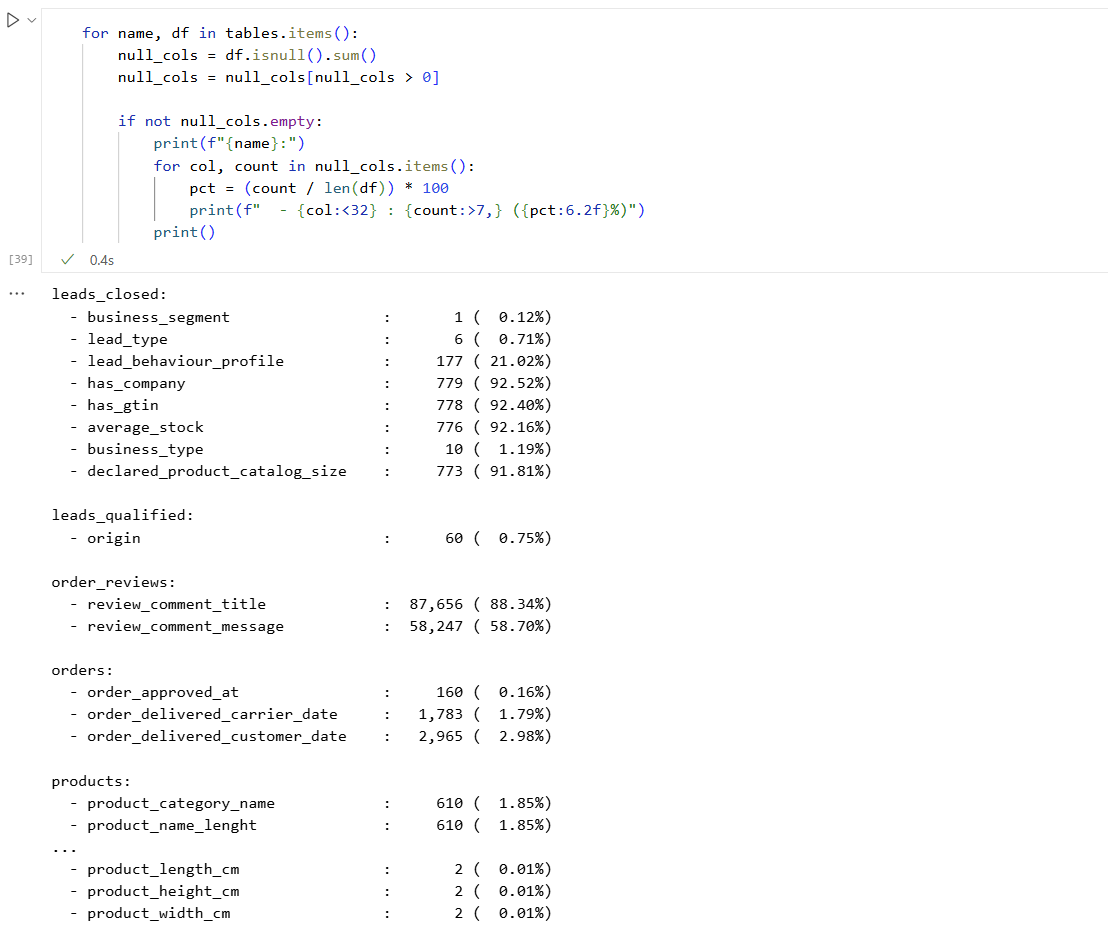
\includegraphics[width=\textwidth]{img_c1/c1_fig04_xu_ly_gia_tri_null.png}
    \caption{Tổng quan phân bố giá trị thiếu trên tất cả bảng dữ liệu thô}
    \label{fig:c1f04}
\end{figure}

\paragraph{Thay thế giá trị thiếu cột nguồn gốc trong bảng khách hàng tiềm năng}

Cột \texttt{origin} trong bảng \texttt{leads\_qualified} là biến phân loại kênh marketing (Organic Search, Paid Search, Social,...). Có 60 dòng bị thiếu thông tin do không ghi nhận được kênh tiếp cận. Giá trị thiếu được thay thế bằng placeholder \texttt{'unknown'} để đảm bảo khi gom nhóm (group-by) đánh giá hiệu quả kênh tiếp thị không bị rơi vào nhóm khuyết danh.

\begin{figure}[H]
    \centering
    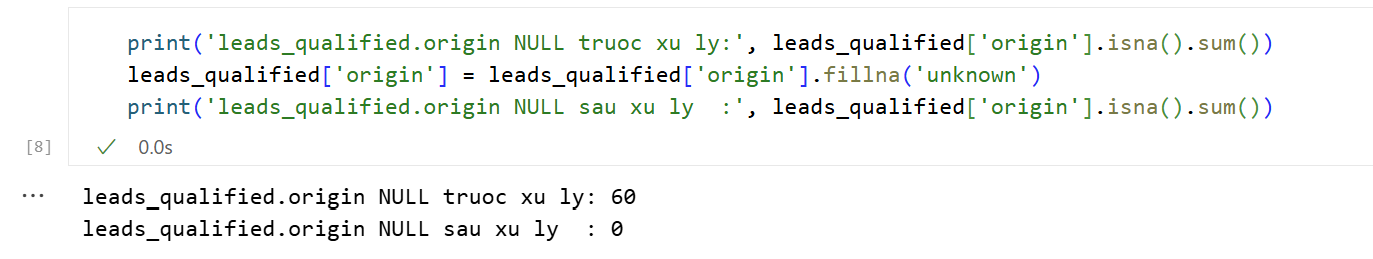
\includegraphics[width=\textwidth]{img_c1/c1_fig05_xu_ly_gia_tri_null.png}
    \caption{Thay thế giá trị thiếu cột nguồn gốc tiếp thị bằng placeholder \texttt{'unknown'}}
    \label{fig:c1f05}
\end{figure}

\paragraph{Giữ nguyên giá trị thiếu các cột biểu mẫu marketing trong bảng chốt hợp đồng}

Các cột như \texttt{business\_segment}, \texttt{lead\_type}, \texttt{lead\_behaviour\_profile}, \texttt{has\_company}, \texttt{average\_stock}, \texttt{declared\_product\_catalog\_size} trong bảng \texttt{leads\_closed} là thông tin do sales rep thu thập thủ công trong quá trình tư vấn và phần lớn là tùy chọn (optional), có tỷ lệ thiếu lên tới 92.5\%.

\begin{quote}\itshape
Về mặt ngữ nghĩa, giá trị thiếu ở đây phản ánh trạng thái \textbf{``chưa thu thập được thông tin''}. Nếu thay thế bằng số 0 cho cột \texttt{average\_stock}, dữ liệu sẽ bị hiểu sai lệch thành đối tác có tồn kho bằng 0. Do đó, việc giữ nguyên \texttt{NaN} là cần thiết để bảo toàn tính trung thực của dữ liệu khảo sát.
\end{quote}

\begin{figure}[H]
    \centering
    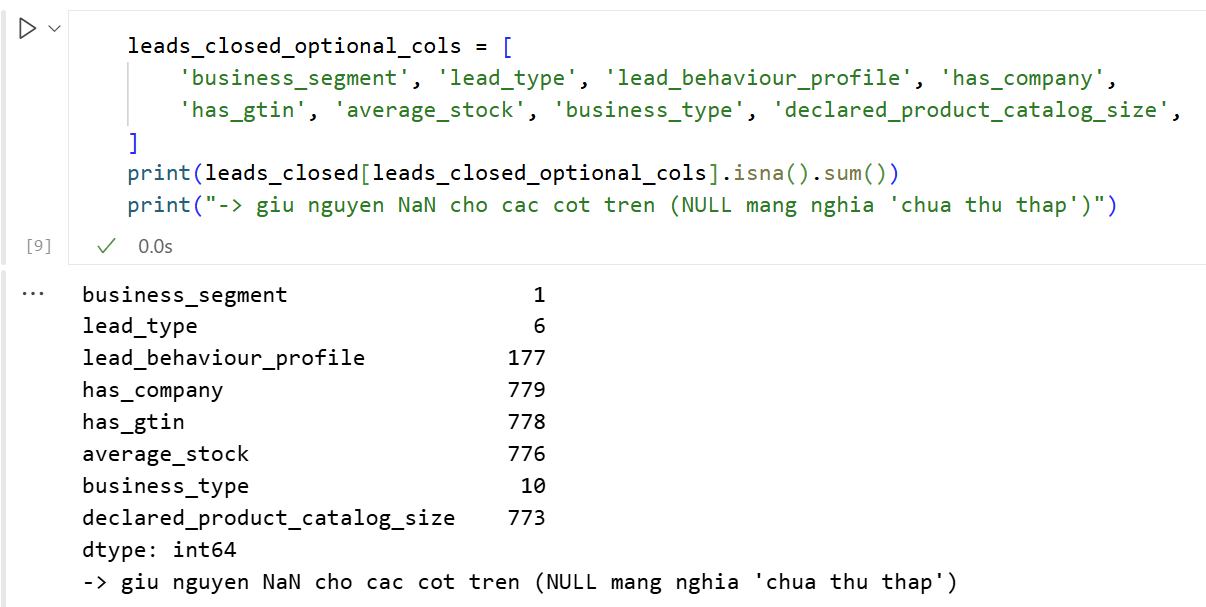
\includegraphics[width=\textwidth]{img_c1/c1_fig06_xu_ly_gia_tri_null.png}
    \caption{Thống kê và bảo toàn giá trị thiếu các cột biểu mẫu marketing trong bảng chốt hợp đồng}
    \label{fig:c1f06}
\end{figure}

\paragraph{Thay thế giá trị thiếu tiêu đề và nội dung nhận xét trong bảng đánh giá}

Cột tiêu đề (\texttt{review\_comment\_title}) có 87.656 dòng thiếu và nội dung (\texttt{review\_comment\_message}) có 58.247 dòng thiếu do khách hàng chỉ chấm điểm sao mà không để lại nhận xét văn bản. Các giá trị thiếu này được điền chuỗi rỗng \texttt{''} bằng phương thức \texttt{fillna('')} để các bước xử lý chuỗi và nạp dữ liệu không gặp lỗi định dạng.

\begin{figure}[H]
    \centering
    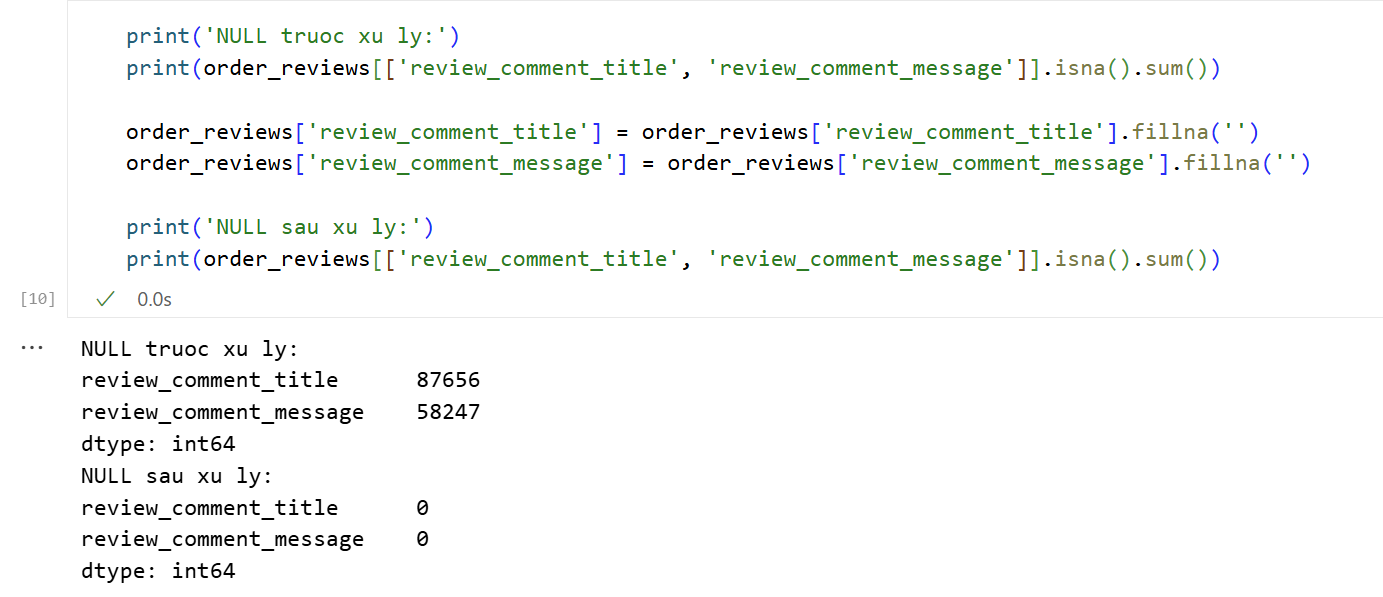
\includegraphics[width=\textwidth]{img_c1/c1_fig07_xu_ly_gia_tri_null.png}
    \caption{Thay thế giá trị thiếu tiêu đề và nội dung nhận xét bằng chuỗi rỗng}
    \label{fig:c1f07}
\end{figure}

\paragraph{Giữ nguyên giá trị thiếu các cột ngày giao hàng và chuyển đổi kiểu dữ liệu}

\begin{itemize}\setlength{\itemsep}{2pt}
  \item Các cột \texttt{order\_approved\_at}, \texttt{order\_delivered\_carrier\_date}, \texttt{order\_delivered\_customer\_date} bị thiếu do đơn hàng \textbf{chưa đi hết chu trình giao hàng} (rơi vào trạng thái bị hủy \texttt{canceled} hoặc hết hàng \texttt{unavailable}).
  \item Giá trị thiếu ở đây là thông tin trạng thái nghiệp vụ thực tế, do đó không thay thế bằng ngày giả định.
  \item Thực hiện chuyển đổi sang kiểu \texttt{datetime64[ns]}, các giá trị thiếu được giữ nguyên dưới dạng \texttt{NaT} để phục vụ tính toán chính xác thời gian vận chuyển (lead time) cho các đơn hàng đã hoàn tất.
\end{itemize}

\begin{figure}[H]
    \centering
    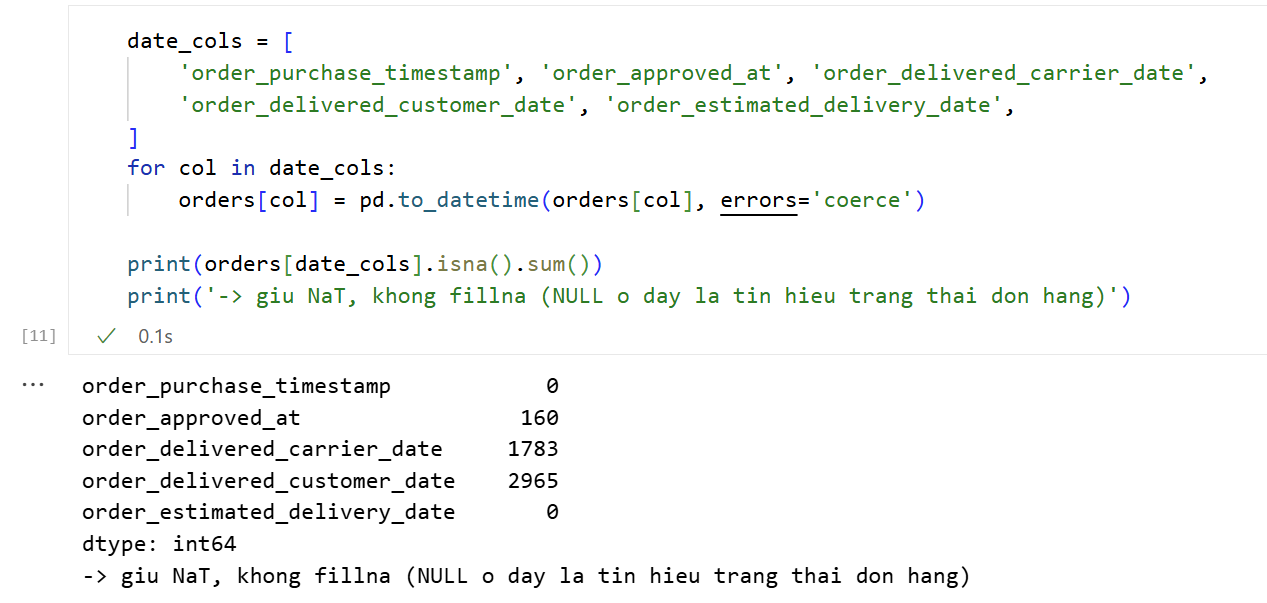
\includegraphics[width=\textwidth]{img_c1/c1_fig08_xu_ly_gia_tri_null.png}
    \caption{Bảo toàn giá trị thiếu các mốc thời gian giao hàng sau khi chuyển đổi kiểu dữ liệu}
    \label{fig:c1f08}
\end{figure}

\paragraph{Xử lý giá trị thiếu theo từng nhóm cột trong bảng sản phẩm}

Bảng \texttt{products} có 610 sản phẩm thiếu thông tin phân loại và kích thước vật lý. Chiến lược xử lý được chia thành 3 nhóm cụ thể trong Bảng~\ref{tab:product_null_strategy}.

\begin{table}[htbp]
\centering
\caption{Quy tắc xử lý giá trị thiếu theo từng nhóm cột trong bảng sản phẩm}\label{tab:product_null_strategy}
\vspace{4pt}
{\footnotesize
\begin{tabular}{@{}p{4.2cm}p{3.5cm}p{6.5cm}@{}}
\toprule
\textbf{Nhóm cột} & \textbf{Cách xử lý} & \textbf{Cơ sở kỹ thuật và nghiệp vụ} \\
\midrule
\texttt{product\_category\_name} & \texttt{fillna('outros')} & Gán vào nhóm danh mục chung ``khác'' (\texttt{outros}) theo chuẩn phân loại tiếng Bồ Đào Nha. \\
\texttt{name\_lenght}, \texttt{description\_lenght}, \texttt{photos\_qty} & \texttt{fillna(0)} & Không có hình ảnh hoặc không có nội dung mô tả tương ứng với giá trị 0. \\
\texttt{weight\_g}, \texttt{length\_cm}, \texttt{height\_cm}, \texttt{width\_cm} & \texttt{fillna(median)} & Phân phối kích thước/trọng lượng bị lệch bởi outlier, dùng giá trị trung vị (median) để không làm méo mó các phân tích logistics. \\
\bottomrule
\end{tabular}}
\end{table}

\begin{figure}[H]
    \centering
    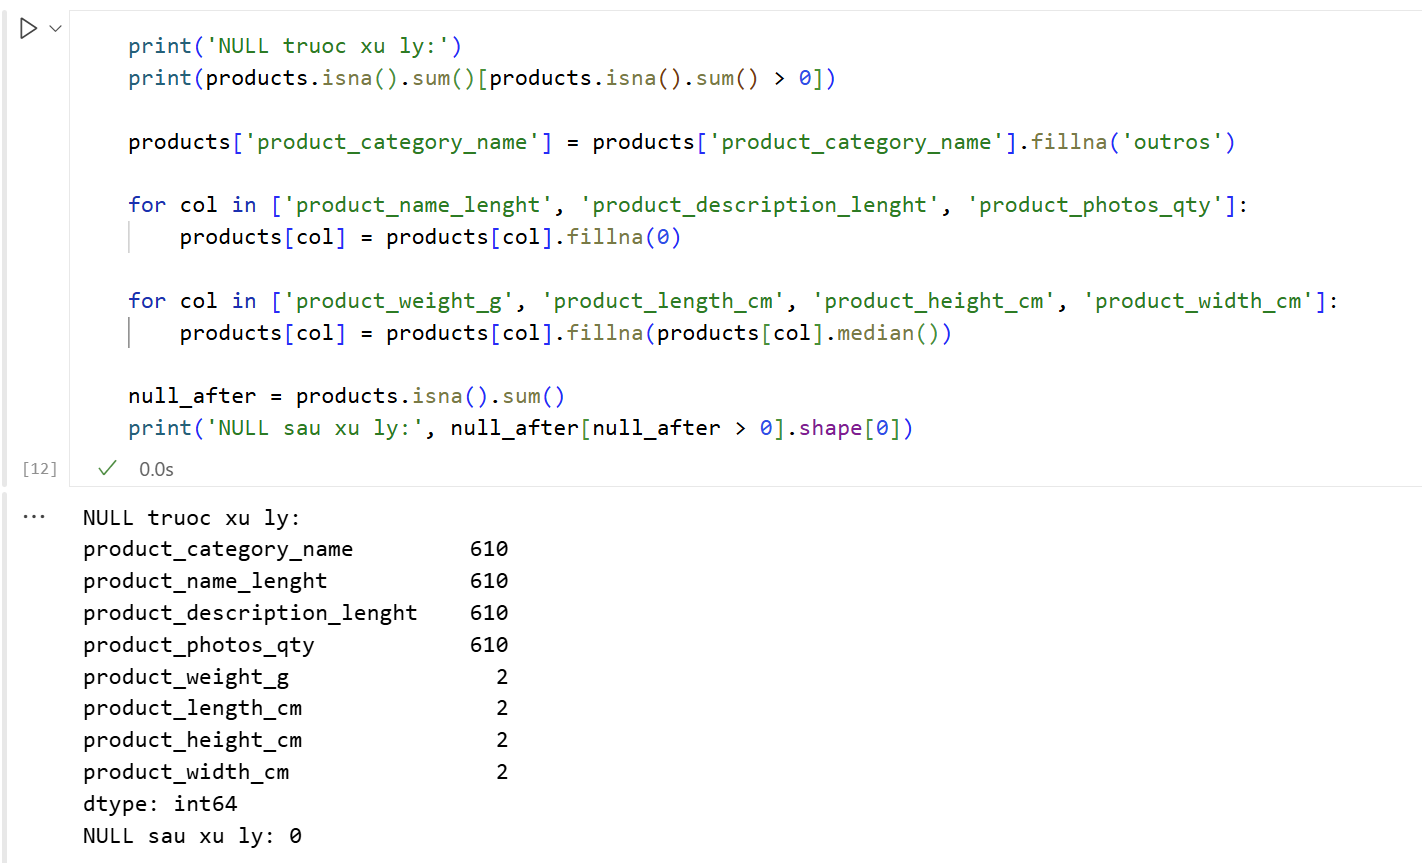
\includegraphics[width=\textwidth]{img_c1/c1_fig09_xu_ly_gia_tri_null.png}
    \caption{Hiện thực hóa xử lý giá trị thiếu trên các nhóm cột trong bảng sản phẩm}
    \label{fig:c1f09}
\end{figure}

\paragraph{Các bảng không có giá trị thiếu}

Kiểm tra xác nhận các bảng \texttt{customers}, \texttt{geolocation}, \texttt{order\_items}, \texttt{order\_payments}, \texttt{sellers} và \texttt{category\_translation} đạt độ hoàn thiện 100\%, không chứa giá trị thiếu cần can thiệp.

\subsubsection{Kiểm tra và xử lý dữ liệu trùng lặp}

Kiểm tra trùng lặp (deduplication) được tiến hành trên từng bảng thô theo cả hai mức độ: trùng lặp khóa chính (PK conflict) và trùng lặp toàn dòng (full-row duplicate), thực hiện trước khi dựng các bảng Dim và Fact.

\begin{figure}[H]
    \centering
    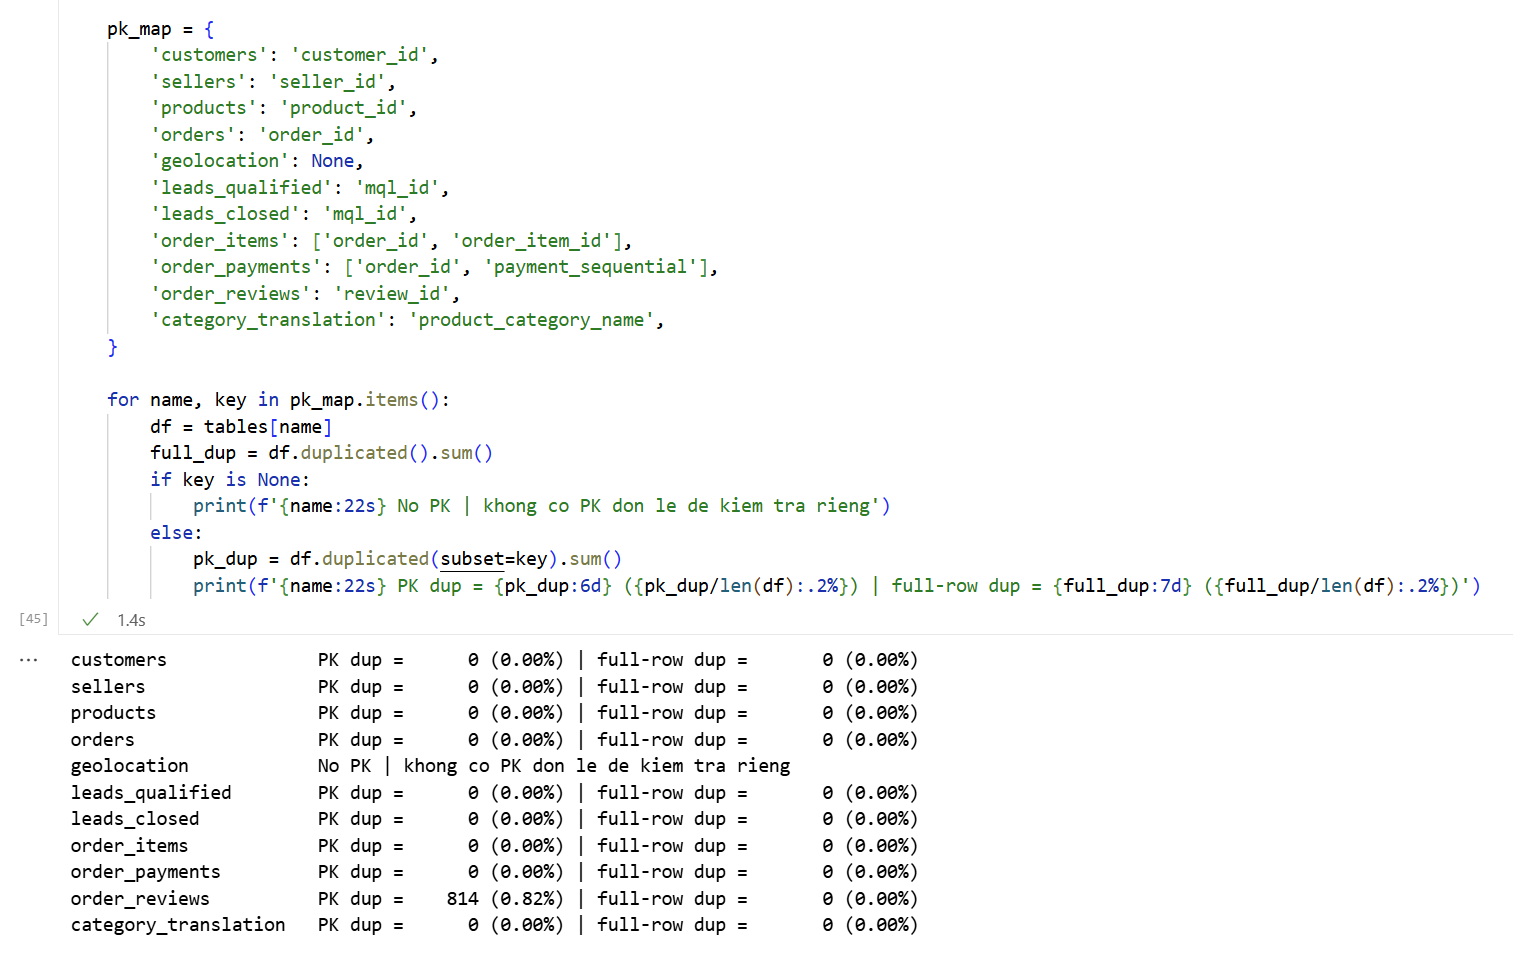
\includegraphics[width=\textwidth]{img_c1/c1_fig10_kiem_tra_xu_ly_du.png}
    \caption{Rà soát bản ghi trùng lặp theo khóa chính và toàn dòng trên tất cả bảng thô}
    \label{fig:c1f10}
\end{figure}

\begin{itemize}\setlength{\itemsep}{2pt}
  \item Kết quả kiểm tra cho thấy bảng \texttt{order\_reviews} có \texttt{full-row duplicate = 0}, nhưng xuất hiện xung đột khóa chính trên cột \texttt{review\_id} ở một số dòng (do khách hàng chỉnh sửa phản hồi hoặc do độ trễ ghi nhận của hệ thống).
  \item Bảng Dim đánh giá yêu cầu mỗi mã \texttt{review\_id} là duy nhất để đảm bảo quan hệ 1-1, do đó áp dụng deduplication giữ lại bản ghi phản hồi đầu tiên.
\end{itemize}

\begin{figure}[H]
    \centering
    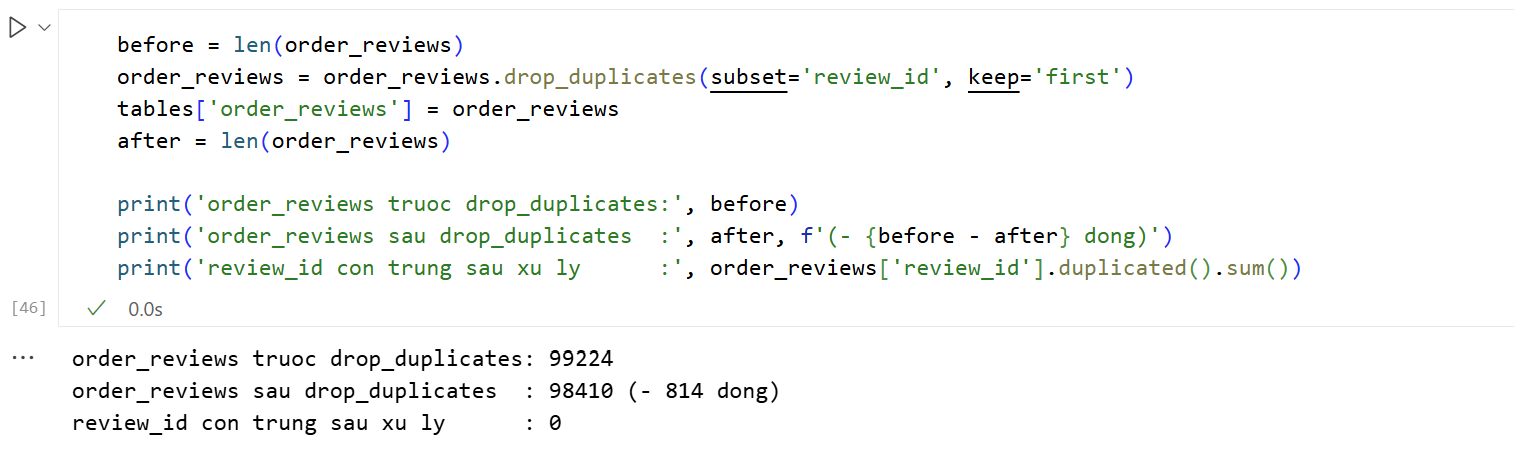
\includegraphics[width=\textwidth]{img_c1/c1_fig11_kiem_tra_xu_ly_du.png}
    \caption{Khử trùng lặp khóa chính \texttt{review\_id} trong bảng đánh giá}
    \label{fig:c1f11}
\end{figure}

\subsubsection{Kiểm tra tính toàn vẹn tham chiếu trên dữ liệu thô}

Kiểm tra khóa ngoại (FK) giữa các bảng thô nhằm phát hiện trước các bản ghi mồ côi (orphan records) cần xử lý khi thiết kế lược đồ.

\paragraph{Kiểm tra sự đầy đủ của danh mục sản phẩm trong bảng dịch danh mục}

Đối chiếu giữa danh mục thực tế trong \texttt{products} và bảng từ điển dịch thuật \texttt{category\_translation} phát hiện có \textbf{3 danh mục sản phẩm} chưa có bản dịch tiếng Anh: \texttt{'outros'} (do vừa điền placeholder), \texttt{'pc\_gamer'} và \texttt{'portateis\_cozinha\_e\_preparadores\_de\_alimentos'}. Vấn đề này được xử lý bổ sung khi xây dựng bảng Dim danh mục.

\begin{figure}[H]
    \centering
    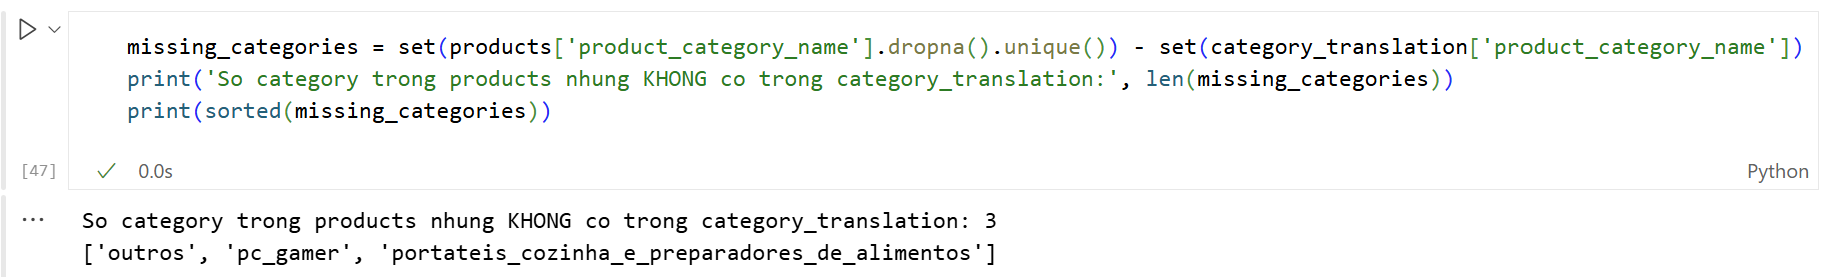
\includegraphics[width=\textwidth]{img_c1/c1_fig12_kiem_tra_referential_integrity_du.png}
    \caption{Kiểm tra sự đầy đủ của danh mục sản phẩm trong bảng dịch danh mục}
    \label{fig:c1f12}
\end{figure}

\paragraph{Kiểm tra sự tồn tại của mã người bán từ bảng chốt hợp đồng trong bảng người bán}

Đối chiếu mã \texttt{seller\_id} giữa bảng chốt hợp đồng (\texttt{leads\_closed}) và bảng người bán (\texttt{sellers}) phát hiện có \textbf{462 / 842 seller\_id (54.87\%)} không tồn tại trong bảng \texttt{sellers}.

\begin{quote}\itshape
\textbf{Nhận xét bản chất nghiệp vụ:} Bảng \texttt{sellers} gốc trong hệ thống thương mại điện tử chỉ lưu trữ các seller đã có ít nhất 01 đơn hàng bán ra thực tế. Trong khi đó, 842 đối tác trong \texttt{leads\_closed} là các lead vừa ký kết hợp đồng (closed deal). Trong số này, 380 seller (45.13\%) đã kích hoạt gian hàng và phát sinh đơn hàng, còn 462 seller (54.87\%) vẫn đang trong giai đoạn tiếp nhận hoặc chưa kịp bán được hàng trong thời gian thu thập dữ liệu. Đây là đặc trưng tự nhiên của phễu chuyển đổi tiếp thị (marketing conversion funnel), không phải lỗi dữ liệu. Do đó, các dòng này được giữ nguyên để phục vụ phân tích tỷ lệ kích hoạt đối tác.
\end{quote}

\begin{figure}[H]
    \centering
    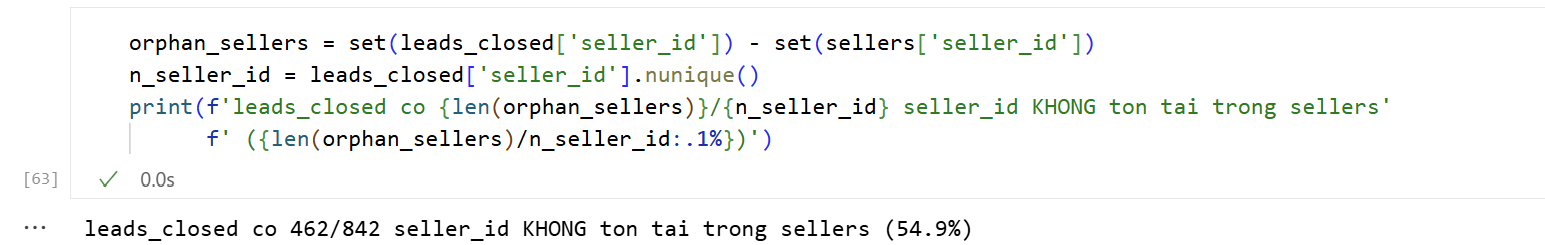
\includegraphics[width=\textwidth]{img_c1/c1_fig13_kiem_tra_referential_integrity_du.png}
    \caption{Kiểm tra đối chiếu mã người bán giữa bảng chốt hợp đồng và bảng người bán}
    \label{fig:c1f13}
\end{figure}

\paragraph{Kiểm tra tính khép kín của mã khách hàng tiềm năng}

Kiểm tra khẳng định 100\% các hợp đồng chốt được trong \texttt{leads\_closed} đều có mã \texttt{mql\_id} xuất phát hợp lệ từ bảng sàng lọc \texttt{leads\_qualified}. Điều này đảm bảo khi thực hiện \texttt{LEFT JOIN} để dựng \texttt{FACT\_SELLER\_LEAD} sẽ không làm thất thoát bất kỳ bản ghi closed deal nào.

\begin{figure}[H]
    \centering
    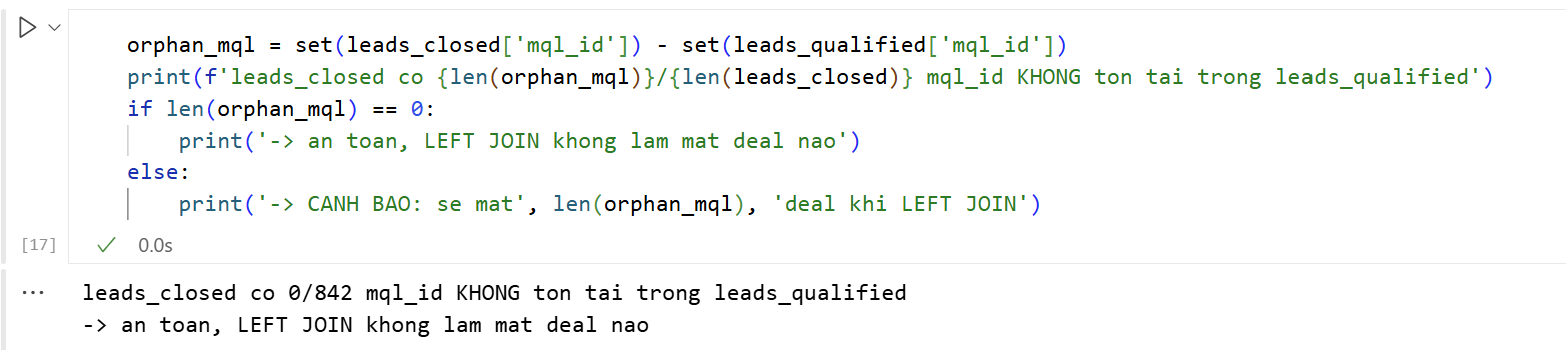
\includegraphics[width=\textwidth]{img_c1/c1_fig14_kiem_tra_referential_integrity_du.png}
    \caption{Xác nhận tính khép kín của định danh khách hàng tiềm năng trong phễu tiếp thị}
    \label{fig:c1f14}
\end{figure}

\subsubsection{Chuẩn hóa mã bưu chính (Zip Code Prefix)}

Mã bưu chính tại Brazil gồm 8 chữ số, trong đó 5 chữ số đầu đại diện cho vùng địa lý đô thị. Do quá trình xuất dữ liệu thô sang kiểu số nguyên (integer), các mã bưu chính có chữ số 0 ở đầu (đặc biệt là khu vực São Paulo) bị mất số 0 dẫn đầu (ví dụ: \texttt{1001} thay vì \texttt{01001}). 

Tiến hành chuẩn hóa toàn bộ tiền tố zip code về chuỗi cố định 5 ký tự bằng hàm \texttt{zfill(5)} trên các bảng \texttt{customers}, \texttt{sellers} và \texttt{geolocation}, giải quyết triệt để lỗi phân mảnh khóa khi thực hiện lookup địa danh.

\begin{figure}[H]
    \centering
    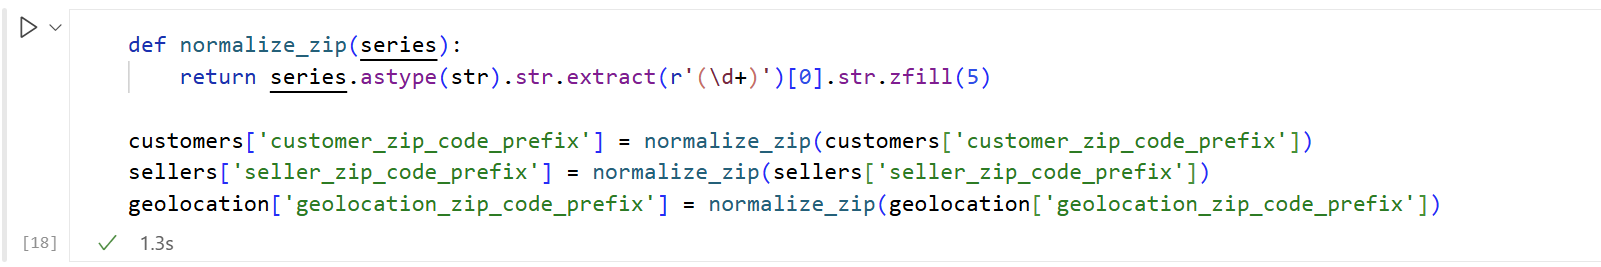
\includegraphics[width=\textwidth]{img_c1/c1_fig15_chuan_hoa_zip_code.png}
    \caption{Chuẩn hóa mã bưu chính về chuỗi ký tự cố định 5 chữ số}
    \label{fig:c1f15}
\end{figure}

% --------------------------------------------------

\subsection{Thiết kế kho dữ liệu}

\subsubsection{Lựa chọn mô hình lược đồ}

Kho dữ liệu được thiết kế theo mô hình \textbf{lược đồ bông tuyết (snowflake schema)}. Khác với lược đồ hình sao vốn giữ mỗi bảng chiều ở dạng một bảng phẳng duy nhất, lược đồ bông tuyết cho phép chuẩn hóa tiếp các phân cấp bên trong bảng chiều thành những bảng con riêng biệt.

Lựa chọn này xuất phát từ hai phân cấp có thật trong dữ liệu Olist:

\begin{itemize}\setlength{\itemsep}{2pt}
  \item \textbf{Danh mục sản phẩm.} Mỗi sản phẩm thuộc một danh mục, và mỗi danh mục có thêm tên tiếng Anh tương ứng. Nếu gộp vào bảng chiều sản phẩm theo lược đồ hình sao, cặp tên danh mục song ngữ sẽ bị lặp lại trên toàn bộ hơn 32 nghìn dòng sản phẩm. Tách thành \texttt{DIM\_PRODUCT\_CATEGORY} giúp mỗi danh mục chỉ được lưu một lần.
  \item \textbf{Địa điểm.} Khách hàng và người bán cùng tham chiếu đến một tập mã bưu chính và tọa độ địa lý. Tách thành \texttt{DIM\_LOCATION} dùng chung cho cả hai bảng chiều giúp tránh nhân đôi hơn một triệu dòng tọa độ, đồng thời bảo đảm hai bảng chiều luôn hiểu địa danh theo cùng một chuẩn.
\end{itemize}

Cần lưu ý rằng lược đồ còn có ba bảng sự kiện khác nhau (chi tiết đơn hàng, lần thanh toán và khách hàng tiềm năng) cùng chia sẻ các bảng chiều, nên xét chặt chẽ đây là một \textit{lược đồ chòm sao} với các bảng chiều đã được bông tuyết hóa. Phần trình bày dưới đây vẫn gọi chung là lược đồ bông tuyết theo đặc trưng nổi bật nhất của thiết kế.

\subsubsection{Lược đồ kho dữ liệu}

Lược đồ đích gồm \textbf{ba bảng sự kiện} và \textbf{sáu bảng chiều}, được thể hiện trong Hình~\ref{fig:c1_luoc_do_kho}.

\texttt{FACT\_ORDER\_ITEMS} giữ vai trò bảng sự kiện trung tâm, liên kết tới ba bảng chiều qua \texttt{customer\_id}, \texttt{seller\_id} và \texttt{product\_id}. Hai nhánh bông tuyết nằm ở phía sau các bảng chiều này: \texttt{DIM\_PRODUCT} trỏ tiếp tới \texttt{DIM\_PRODUCT\_CATEGORY} qua \texttt{product\_category\_name}, còn \texttt{DIM\_CUSTOMER} và \texttt{DIM\_SELLER} cùng trỏ tới \texttt{DIM\_LOCATION} qua khóa thay thế \texttt{location\_id}.

Ba quan hệ còn lại không đi qua bảng chiều: \texttt{FACT\_ORDER\_PAYMENT} và \texttt{DIM\_REVIEW} cùng tham chiếu \texttt{order\_id} của \texttt{FACT\_ORDER\_ITEMS}, còn \texttt{FACT\_SELLER\_LEAD} tham chiếu \texttt{seller\_id} của \texttt{DIM\_SELLER}. Toàn bộ lược đồ dùng khóa tự nhiên của dữ liệu gốc, ngoại trừ \texttt{location\_id} là khóa thay thế được sinh thêm vì tiền tố mã bưu chính không có tính duy nhất trong bảng tọa độ.

\begin{figure}[H]
    \centering
    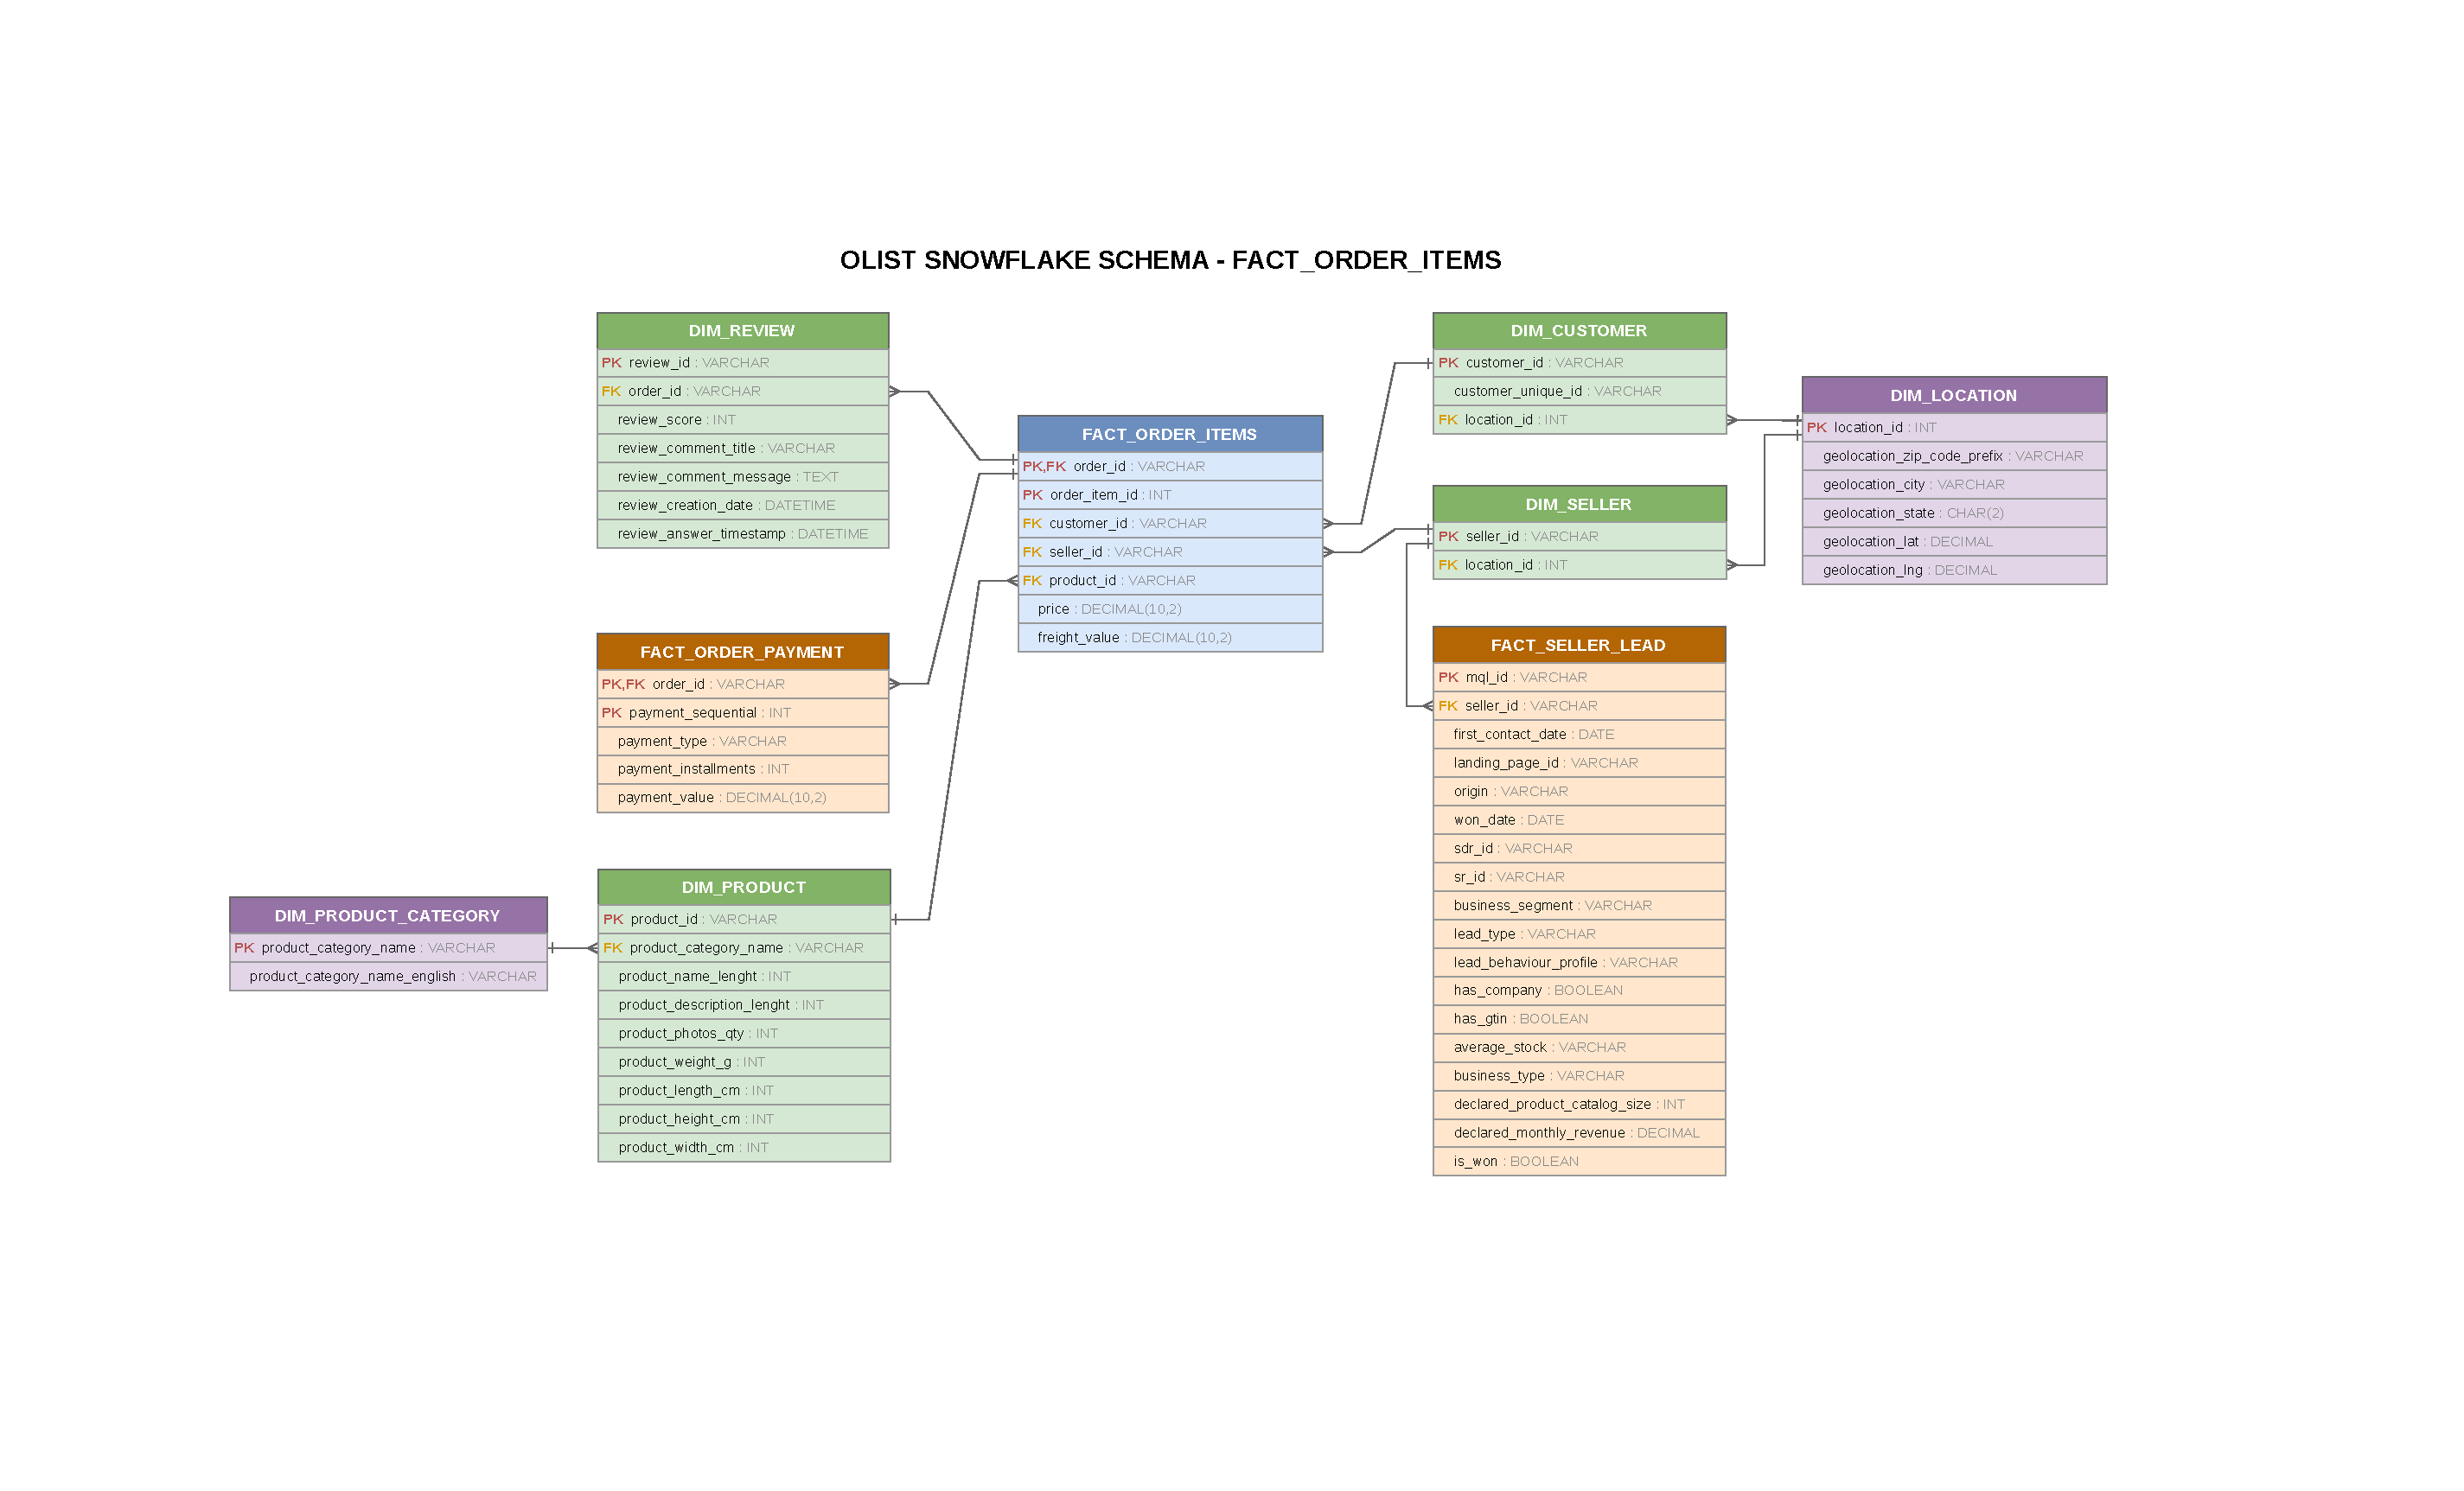
\includegraphics[width=\textwidth]{img_c1/c1_fig26_luoc_do_kho_du_lieu.pdf}
    \caption{Lược đồ bông tuyết của kho dữ liệu Olist sau tiền xử lý}
    \label{fig:c1_luoc_do_kho}
\end{figure}

\subsubsection{Xây dựng và mô tả chi tiết các bảng Chiều (Dimension Tables)}

Để bảo đảm tính toàn vẹn tham chiếu khóa ngoại, các bảng chiều (Dimension) được tạo trước từ dữ liệu nguồn đã qua làm sạch để làm cơ sở tra cứu cho các bảng sự kiện. Dưới đây là quy trình xây dựng, cài đặt và từ điển dữ liệu chi tiết cho từng bảng chiều theo thứ tự phụ thuộc.

\paragraph{Bảng chiều địa điểm (DIM\_LOCATION)}

Bảng \texttt{DIM\_LOCATION} giữ nguyên toàn bộ 1.000.163 dòng tọa độ gốc để bảo toàn thông tin không gian, bổ sung thêm khóa thay thế tự tăng \texttt{location\_id} (Surrogate Key) từ 1 đến $N$. Do tiền tố mã bưu chính (\texttt{geolocation\_zip\_code\_prefix}) không có tính duy nhất trong bảng tọa độ (một mã zip có thể ứng với nhiều điểm khảo sát tọa độ khác nhau), các bảng chiều khách hàng và người bán sẽ thực hiện liên kết thông qua khóa thay thế \texttt{location\_id} này.

\begin{figure}[H]
    \centering
    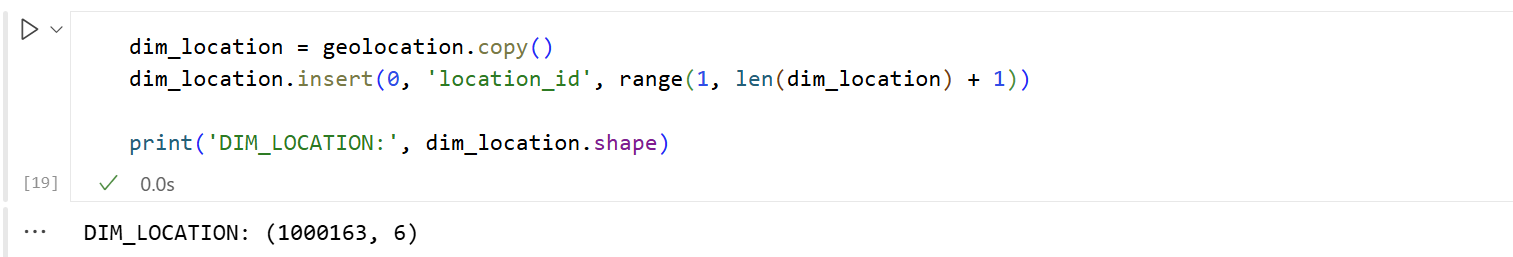
\includegraphics[width=\textwidth]{img_c1/c1_fig16_dim_location.png}
    \caption{Hiện thực hóa xây dựng bảng chiều địa điểm \texttt{DIM\_LOCATION}}
    \label{fig:c1f16}
\end{figure}

{\footnotesize
\begin{longtable}{@{}p{4.7cm}p{2.1cm}p{8.2cm}@{}}
\caption{Các thuộc tính của bảng \texttt{DIM\_LOCATION}}\label{tab:dimlocation}\\
\toprule
\textbf{Tên thuộc tính} & \textbf{Kiểu dữ liệu} & \textbf{Ý nghĩa}\\
\midrule
\endfirsthead
\multicolumn{3}{@{}l}{\textit{Bảng \ref{tab:dimlocation} (tiếp theo)}}\\
\toprule
\textbf{Tên thuộc tính} & \textbf{Kiểu dữ liệu} & \textbf{Ý nghĩa}\\
\midrule
\endhead
\midrule
\multicolumn{3}{r@{}}{\textit{(xem tiếp trang sau)}}\\
\endfoot
\bottomrule
\endlastfoot
\texttt{location\_id} & integer & Khóa chính thay thế của bảng chiều địa điểm, đánh số tuần tự\\
\texttt{geolocation\_zip\_code\_prefix} & string & Năm chữ số đầu của mã bưu chính, đã chuẩn hóa thành chuỗi 5 ký tự\\
\texttt{geolocation\_lat} & float & Vĩ độ của điểm tọa độ\\
\texttt{geolocation\_lng} & float & Kinh độ của điểm tọa độ\\
\texttt{geolocation\_city} & string & Tên thành phố ứng với tọa độ\\
\texttt{geolocation\_state} & string & Mã bang ứng với tọa độ\\
\end{longtable}}

\paragraph{Bảng chiều danh mục sản phẩm (DIM\_PRODUCT\_CATEGORY)}

Bảng \texttt{DIM\_PRODUCT\_CATEGORY} được xây dựng từ bảng \texttt{category\_translation}, bổ sung thêm 3 danh mục còn thiếu đã phát hiện ở bước~\ref{subsec:tienxuly} (bao gồm cả \texttt{'outros'}). Đối với các danh mục bổ sung, sử dụng chính tên gốc tiếng Bồ Đào Nha làm placeholder cho cột tiếng Anh, tạo thành từ điển phân loại hoàn chỉnh gồm 74 dòng.

\begin{figure}[H]
    \centering
    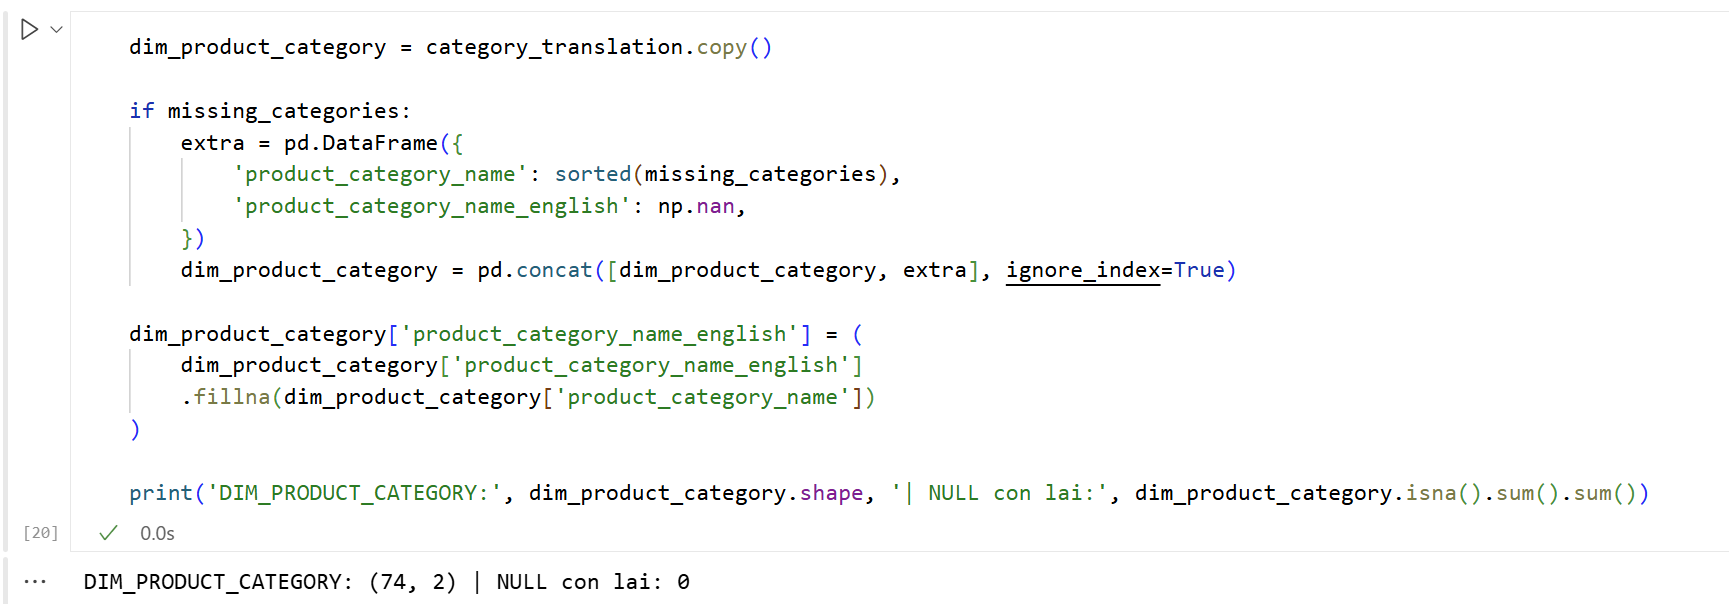
\includegraphics[width=\textwidth]{img_c1/c1_fig17_dim_product_category.png}
    \caption{Xây dựng bảng chiều danh mục sản phẩm song ngữ}
    \label{fig:c1f17}
\end{figure}

{\footnotesize
\begin{longtable}{@{}p{4.7cm}p{2.1cm}p{8.2cm}@{}}
\caption{Các thuộc tính của bảng \texttt{DIM\_PRODUCT\_CATEGORY}}\label{tab:dimproductcategory}\\
\toprule
\textbf{Tên thuộc tính} & \textbf{Kiểu dữ liệu} & \textbf{Ý nghĩa}\\
\midrule
\endfirsthead
\multicolumn{3}{@{}l}{\textit{Bảng \ref{tab:dimproductcategory} (tiếp theo)}}\\
\toprule
\textbf{Tên thuộc tính} & \textbf{Kiểu dữ liệu} & \textbf{Ý nghĩa}\\
\midrule
\endhead
\midrule
\multicolumn{3}{r@{}}{\textit{(xem tiếp trang sau)}}\\
\endfoot
\bottomrule
\endlastfoot
\texttt{product\_category\_name} & string & Tên danh mục sản phẩm bằng tiếng Bồ Đào Nha, khóa chính\\
\texttt{product\_category\_name\_english} & string & Tên danh mục tương ứng bằng tiếng Anh\\
\end{longtable}}

\paragraph{Bảng chiều sản phẩm (DIM\_PRODUCT)}

Bảng \texttt{DIM\_PRODUCT} gồm 32.951 sản phẩm duy nhất với 9 thuộc tính mô tả đặc tính vật lý và danh mục sản phẩm đã được làm sạch ở bước xử lý giá trị khuyết thiếu. Bảng liên kết khóa ngoại \texttt{product\_category\_name} tới bảng \texttt{DIM\_PRODUCT\_CATEGORY}.

\begin{figure}[H]
    \centering
    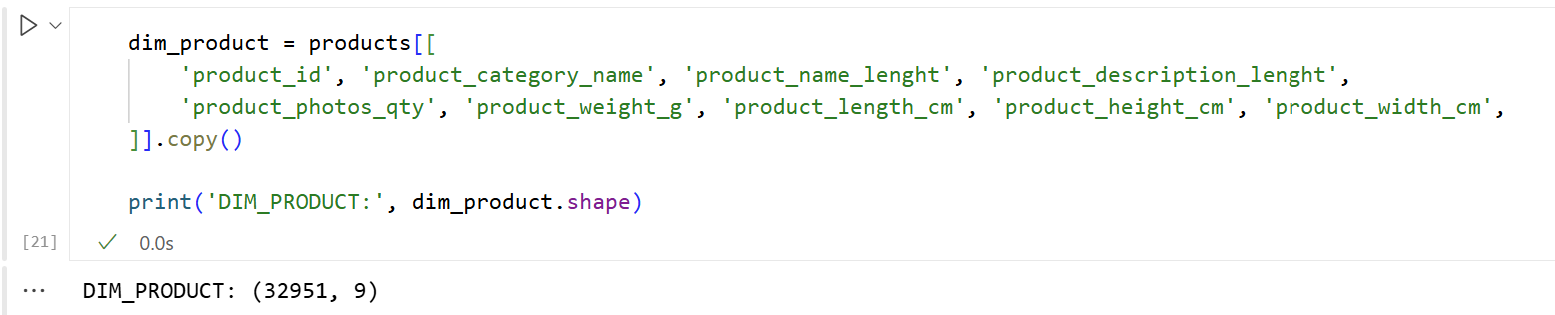
\includegraphics[width=\textwidth]{img_c1/c1_fig18_dim_product.png}
    \caption{Cấu trúc bảng chiều sản phẩm sau khi làm sạch}
    \label{fig:c1f18}
\end{figure}

{\footnotesize
\begin{longtable}{@{}p{4.7cm}p{2.1cm}p{8.2cm}@{}}
\caption{Các thuộc tính của bảng \texttt{DIM\_PRODUCT}}\label{tab:dimproduct}\\
\toprule
\textbf{Tên thuộc tính} & \textbf{Kiểu dữ liệu} & \textbf{Ý nghĩa}\\
\midrule
\endfirsthead
\multicolumn{3}{@{}l}{\textit{Bảng \ref{tab:dimproduct} (tiếp theo)}}\\
\toprule
\textbf{Tên thuộc tính} & \textbf{Kiểu dữ liệu} & \textbf{Ý nghĩa}\\
\midrule
\endhead
\midrule
\multicolumn{3}{r@{}}{\textit{(xem tiếp trang sau)}}\\
\endfoot
\bottomrule
\endlastfoot
\texttt{product\_id} & string & Mã sản phẩm, khóa chính\\
\texttt{product\_category\_name} & string & Tên danh mục sản phẩm bằng tiếng Bồ Đào Nha, khóa chính (khóa ngoại tới \texttt{DIM\_PRODUCT\_CATEGORY})\\
\texttt{product\_name\_lenght} & float & Số ký tự trong tên sản phẩm\\
\texttt{product\_description\_lenght} & float & Số ký tự trong phần mô tả sản phẩm\\
\texttt{product\_photos\_qty} & float & Số lượng ảnh đăng kèm sản phẩm\\
\texttt{product\_weight\_g} & float & Khối lượng sản phẩm, đơn vị gam\\
\texttt{product\_length\_cm} & float & Chiều dài kiện hàng, đơn vị cm\\
\texttt{product\_height\_cm} & float & Chiều cao kiện hàng, đơn vị cm\\
\texttt{product\_width\_cm} & float & Chiều rộng kiện hàng, đơn vị cm\\
\end{longtable}}

\paragraph{Bảng chiều khách hàng (DIM\_CUSTOMER)}

Bảng \texttt{DIM\_CUSTOMER} định danh khách hàng gắn với từng đơn hàng (\texttt{customer\_id}) và người mua duy nhất (\texttt{customer\_unique\_id}). Để ánh xạ chính xác khóa ngoại \texttt{location\_id} từ bảng địa điểm cho khách hàng mà không để lại giá trị khuyết, quy trình lookup phân cấp 3 bước được áp dụng:
\begin{enumerate}\setlength{\itemsep}{2pt}
  \item \textbf{Bước 1 (Khớp chính xác bộ ba):} Chuẩn hóa tên thành phố, bang và thực hiện join theo bộ ba giá trị \texttt{(zip, city, state)} sau khi chuyển về chữ thường.
  \item \textbf{Bước 2 (Fallback lookup theo Zip):} Với các dòng không khớp do sai lệch ký tự tên thành phố, áp dụng phương án dự phòng lookup chỉ theo mã \texttt{zip}.
  \item \textbf{Bước 3 (Bổ sung địa danh mới):} Với số lượng nhỏ khách hàng có mã bưu chính hoàn toàn chưa xuất hiện trong bảng khảo sát tọa độ, hệ thống tự động chèn dòng địa danh mới vào \texttt{DIM\_LOCATION} (với tọa độ để trống) và gán ngược lại \texttt{location\_id}.
\end{enumerate}
Quy trình này bảo đảm 100\% khách hàng đều có khóa ngoại \texttt{location\_id} hợp lệ, đạt tỷ lệ orphan 0\%.

\begin{figure}[H]
    \centering
    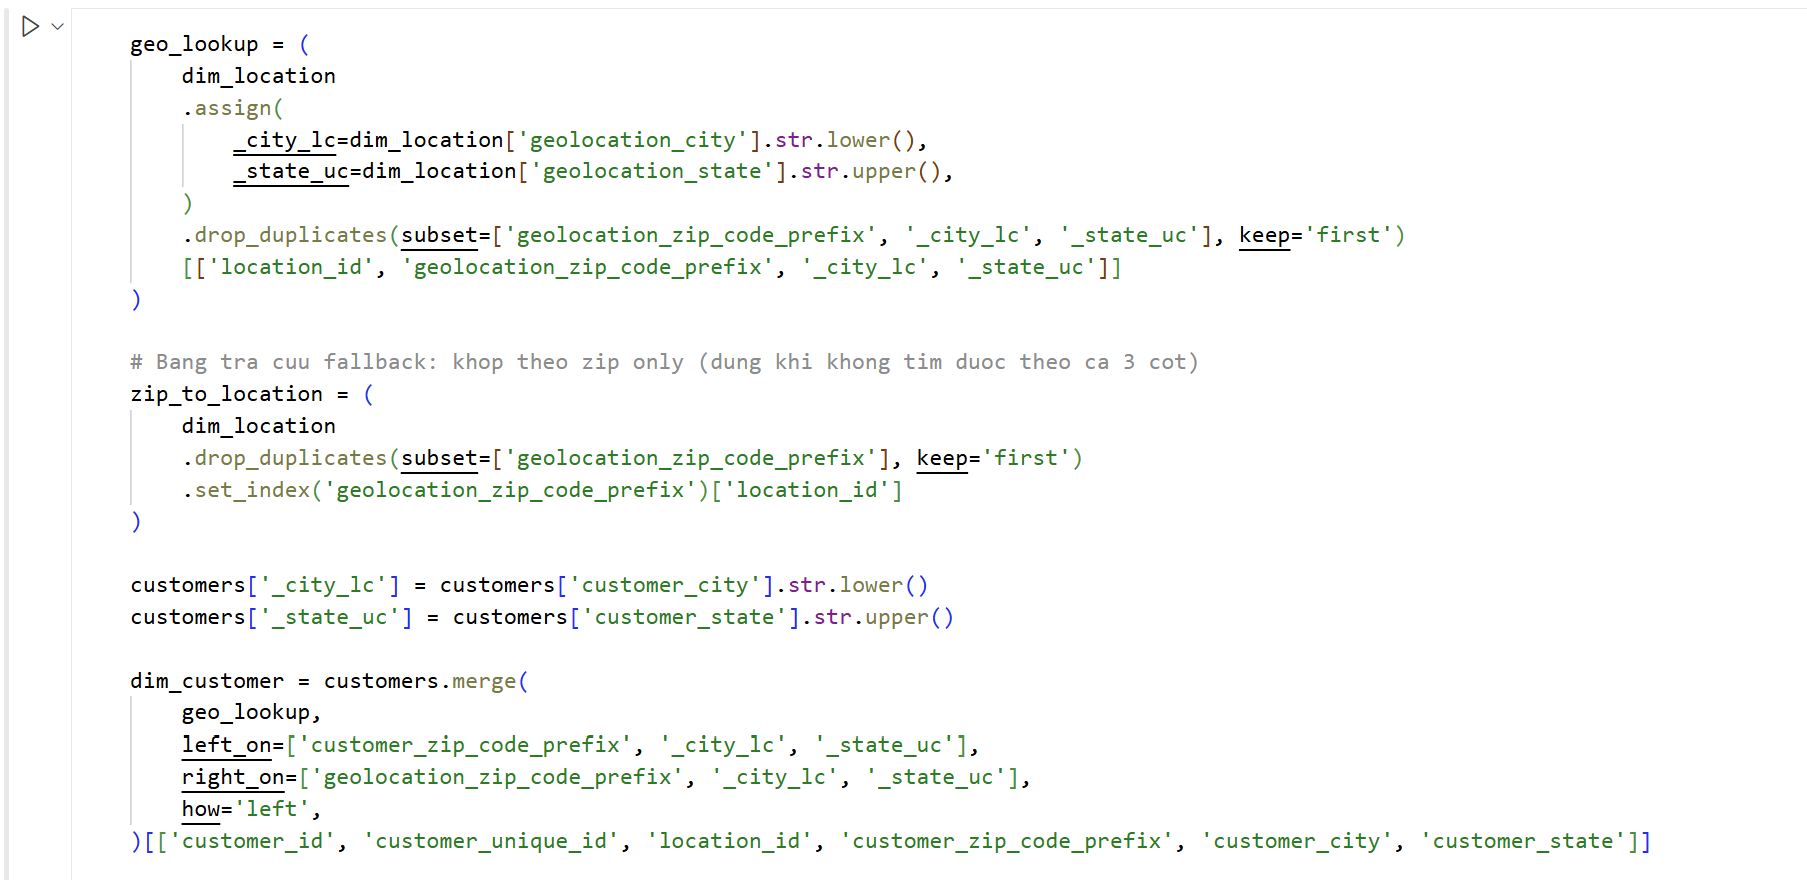
\includegraphics[width=\textwidth]{img_c1/c1_fig19a_dim_customer.png}
    \caption{Quy trình ánh xạ khóa địa điểm cho bảng chiều khách hàng (Bước 1)}
    \label{fig:c1f19a}
\end{figure}

\begin{figure}[H]
    \centering
    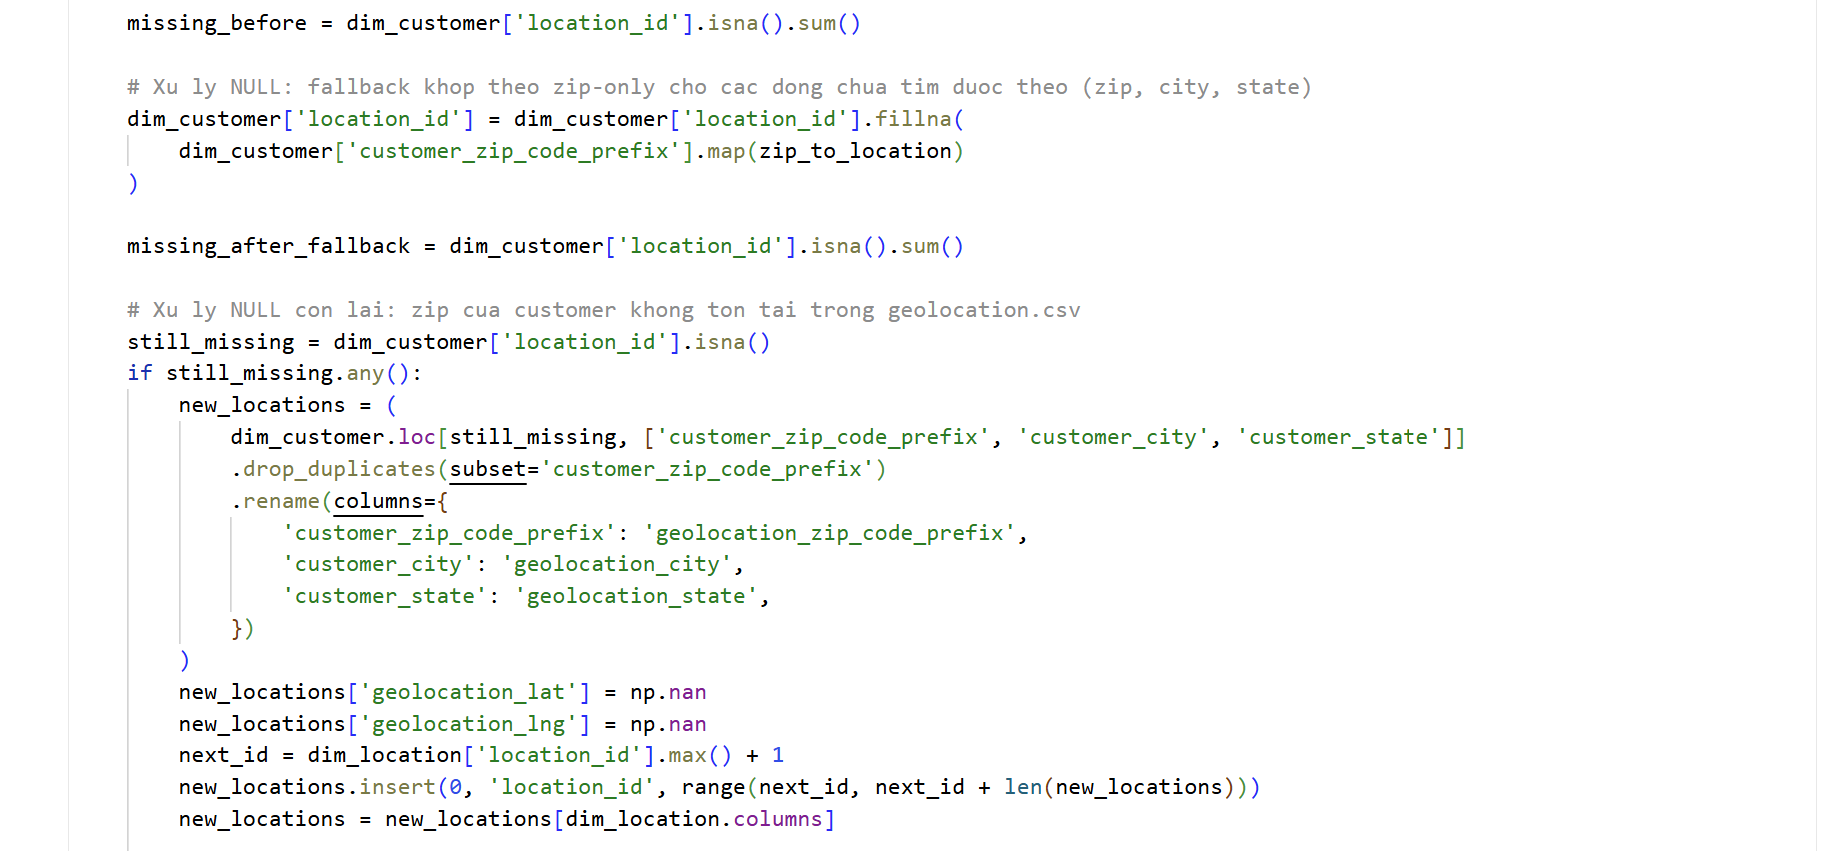
\includegraphics[width=\textwidth]{img_c1/c1_fig19b_dim_customer.png}
    \caption{Thực hiện fallback lookup và bổ sung địa danh cho khách hàng (Bước 2)}
    \label{fig:c1f19b}
\end{figure}

\begin{figure}[H]
    \centering
    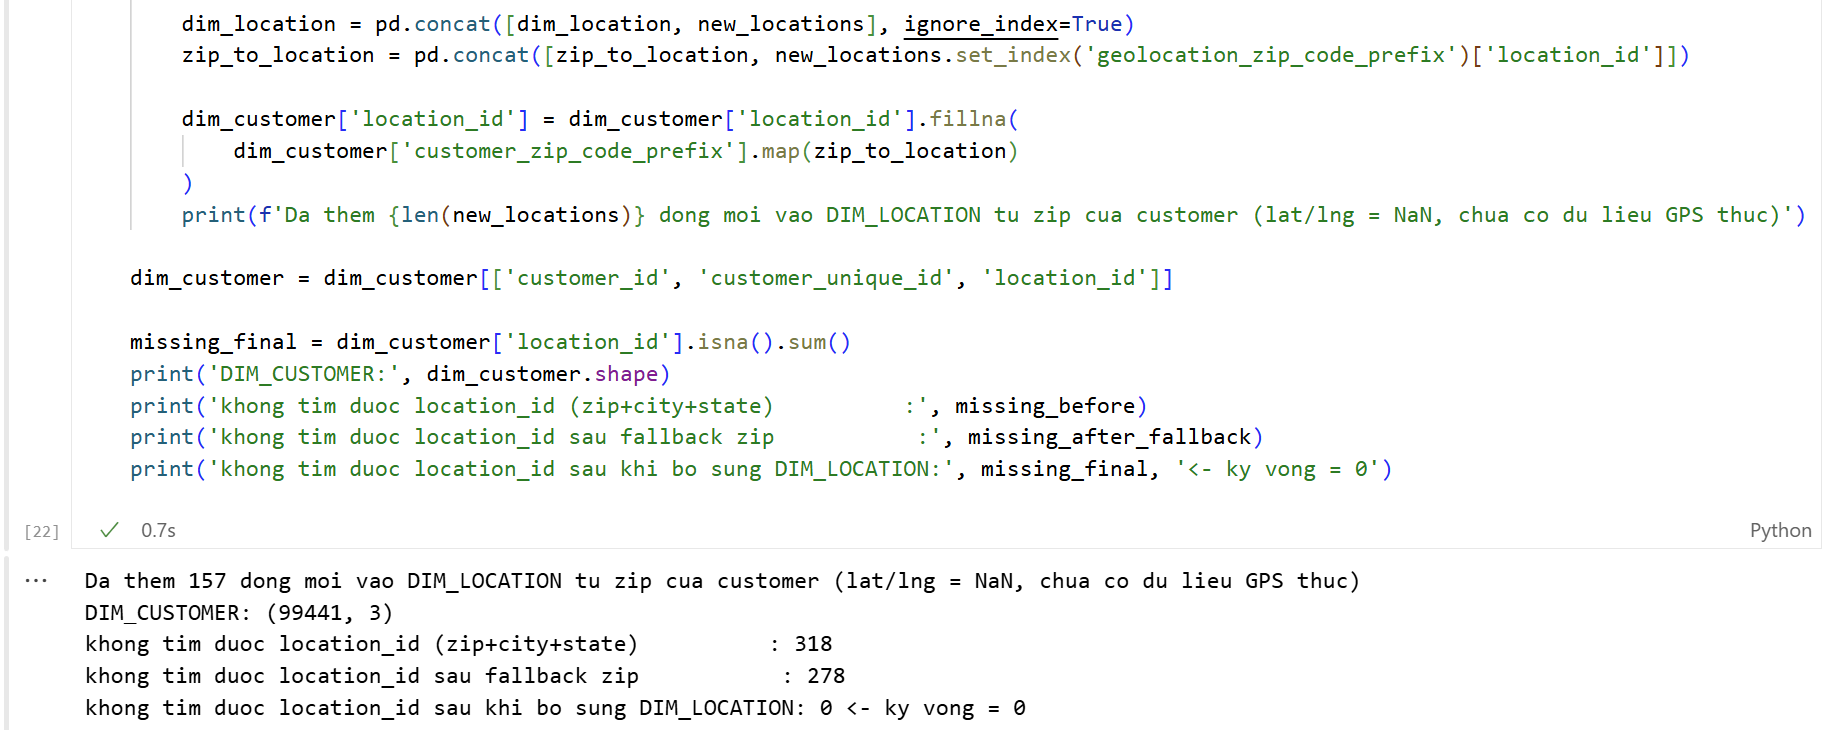
\includegraphics[width=\textwidth]{img_c1/c1_fig19c_dim_customer.png}
    \caption{Xác nhận toàn vẹn khóa ngoại \texttt{location\_id} trên bảng khách hàng (Bước 3)}
    \label{fig:c1f19c}
\end{figure}

{\footnotesize
\begin{longtable}{@{}p{4.7cm}p{2.1cm}p{8.2cm}@{}}
\caption{Các thuộc tính của bảng \texttt{DIM\_CUSTOMER}}\label{tab:dimcustomer}\\
\toprule
\textbf{Tên thuộc tính} & \textbf{Kiểu dữ liệu} & \textbf{Ý nghĩa}\\
\midrule
\endfirsthead
\multicolumn{3}{@{}l}{\textit{Bảng \ref{tab:dimcustomer} (tiếp theo)}}\\
\toprule
\textbf{Tên thuộc tính} & \textbf{Kiểu dữ liệu} & \textbf{Ý nghĩa}\\
\midrule
\endhead
\midrule
\multicolumn{3}{r@{}}{\textit{(xem tiếp trang sau)}}\\
\endfoot
\bottomrule
\endlastfoot
\texttt{customer\_id} & string & Mã khách hàng gắn với từng đơn hàng, khóa chính\\
\texttt{customer\_unique\_id} & string & Mã nhận diện duy nhất của một người mua, dùng để phát hiện khách mua lặp lại\\
\texttt{location\_id} & float & Khóa chính thay thế của bảng chiều địa điểm, đánh số tuần tự (khóa ngoại tới \texttt{DIM\_LOCATION})\\
\end{longtable}}

\paragraph{Bảng chiều người bán (DIM\_SELLER)}

Bảng \texttt{DIM\_SELLER} định danh người bán (\texttt{seller\_id}). Tương tự bảng khách hàng, quy trình lookup phân cấp 3 bước được áp dụng bằng cách tái sử dụng bảng tra cứu \texttt{zip\_to\_location} đã hoàn thiện. Toàn bộ 3.095 người bán đều được gán \texttt{location\_id} thành công mà không để lại giá trị NULL.

\begin{figure}[H]
    \centering
    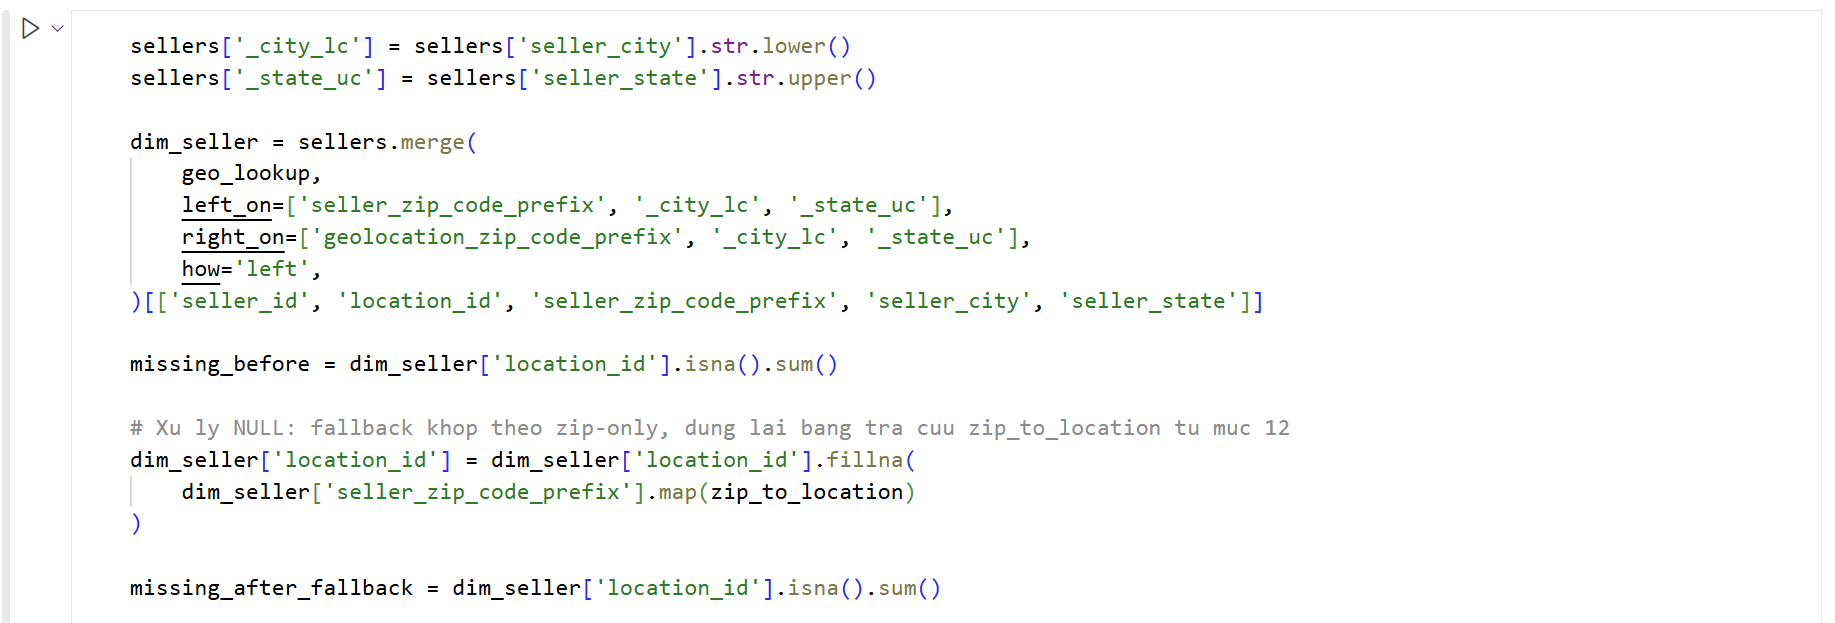
\includegraphics[width=\textwidth]{img_c1/c1_fig20a_dim_seller.png}
    \caption{Ánh xạ khóa địa điểm cho bảng chiều người bán (Phần 1)}
    \label{fig:c1f20a}
\end{figure}

\begin{figure}[H]
    \centering
    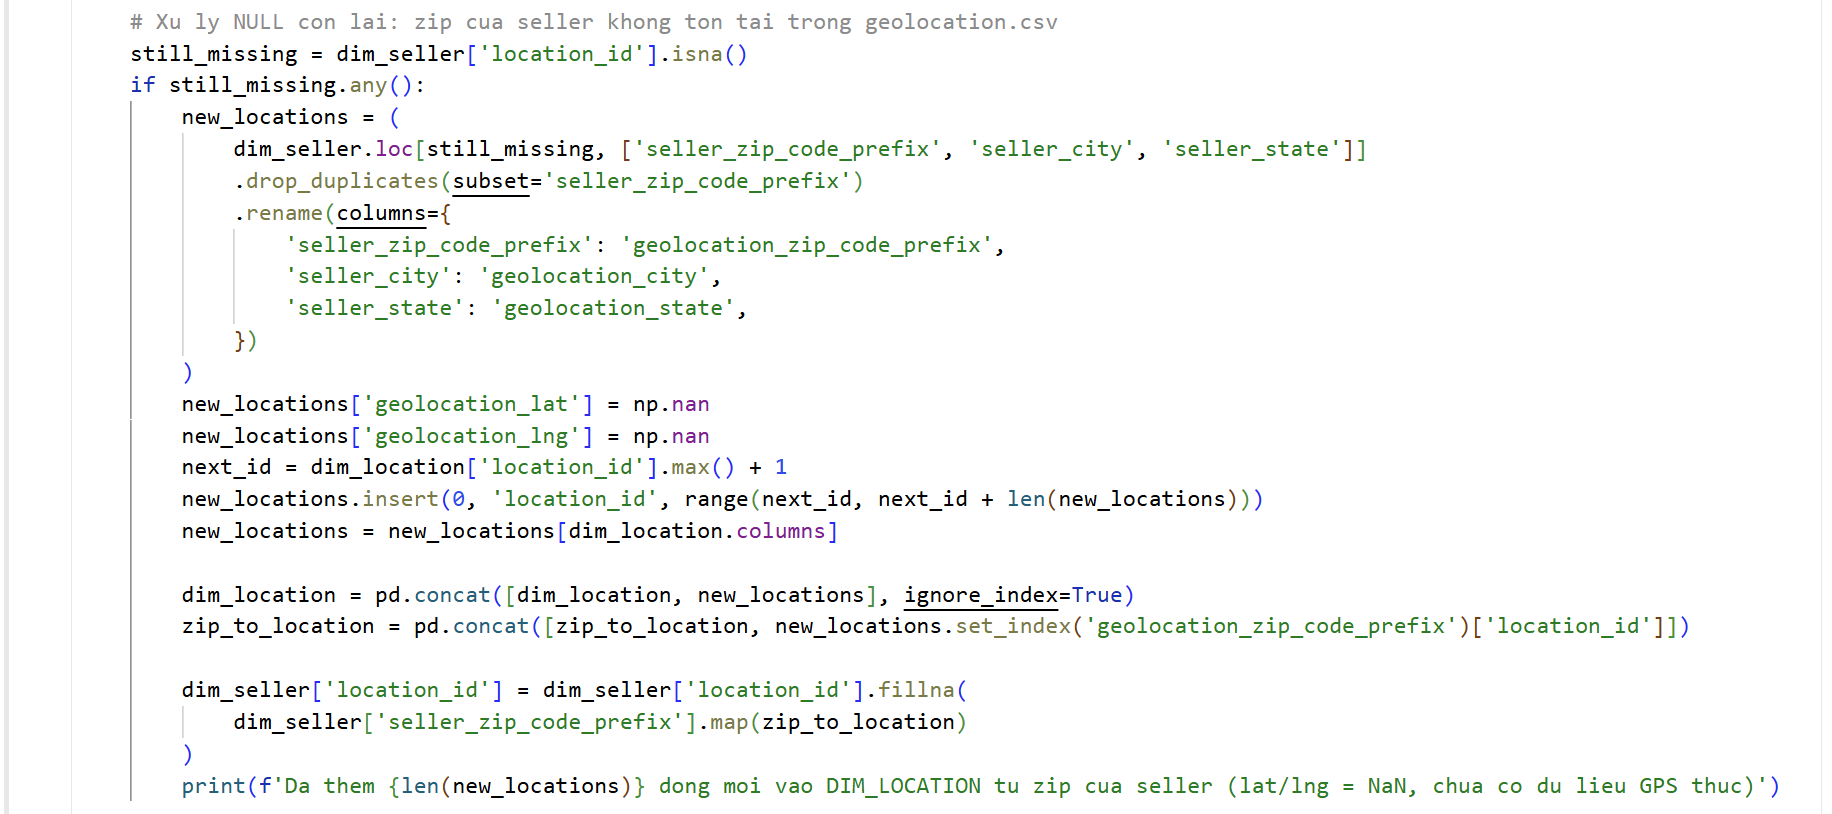
\includegraphics[width=\textwidth]{img_c1/c1_fig20b_dim_seller.png}
    \caption{Ánh xạ khóa địa điểm cho bảng chiều người bán (Phần 2)}
    \label{fig:c1f20b}
\end{figure}

\begin{figure}[H]
    \centering
    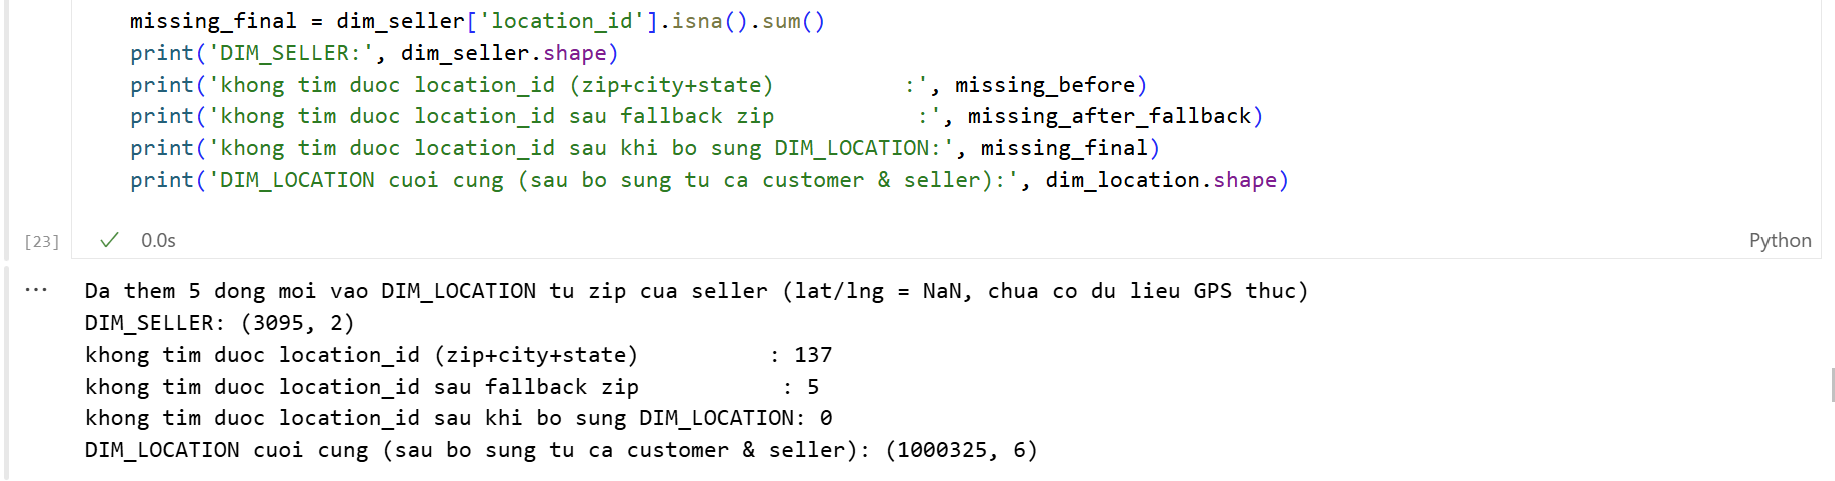
\includegraphics[width=\textwidth]{img_c1/c1_fig20c_dim_seller.png}
    \caption{Khẳng định tính hoàn thiện không khuyết thiếu của khóa ngoại ở bảng chiều người bán}
    \label{fig:c1f20c}
\end{figure}

{\footnotesize
\begin{longtable}{@{}p{4.7cm}p{2.1cm}p{8.2cm}@{}}
\caption{Các thuộc tính của bảng \texttt{DIM\_SELLER}}\label{tab:dimseller}\\
\toprule
\textbf{Tên thuộc tính} & \textbf{Kiểu dữ liệu} & \textbf{Ý nghĩa}\\
\midrule
\endfirsthead
\multicolumn{3}{@{}l}{\textit{Bảng \ref{tab:dimseller} (tiếp theo)}}\\
\toprule
\textbf{Tên thuộc tính} & \textbf{Kiểu dữ liệu} & \textbf{Ý nghĩa}\\
\midrule
\endhead
\midrule
\multicolumn{3}{r@{}}{\textit{(xem tiếp trang sau)}}\\
\endfoot
\bottomrule
\endlastfoot
\texttt{seller\_id} & string & Mã người bán, khóa chính\\
\texttt{location\_id} & float & Khóa chính thay thế của bảng chiều địa điểm, đánh số tuần tự (khóa ngoại tới \texttt{DIM\_LOCATION})\\
\end{longtable}}

\paragraph{Bảng chiều đánh giá (DIM\_REVIEW)}

Bảng \texttt{DIM\_REVIEW} lưu trữ 98.410 phiếu đánh giá trải nghiệm dịch vụ của khách hàng. Quá trình xử lý bao gồm:
\begin{itemize}\setlength{\itemsep}{2pt}
  \item Khử trùng lặp khóa chính \texttt{review\_id} (giữ lại bản ghi phản hồi đầu tiên).
  \item Chuyển đổi các cột ngày tạo phiếu (\texttt{review\_creation\_date}) và thời điểm trả lời (\texttt{review\_answer\_timestamp}) sang kiểu thời gian (\texttt{datetime}).
  \item Tiêu đề và nội dung nhận xét khuyết thiếu đã được thay thế bằng chuỗi rỗng ở bước làm sạch dữ liệu, liên kết tới đơn hàng qua khóa ngoại \texttt{order\_id}.
\end{itemize}

\begin{figure}[H]
    \centering
    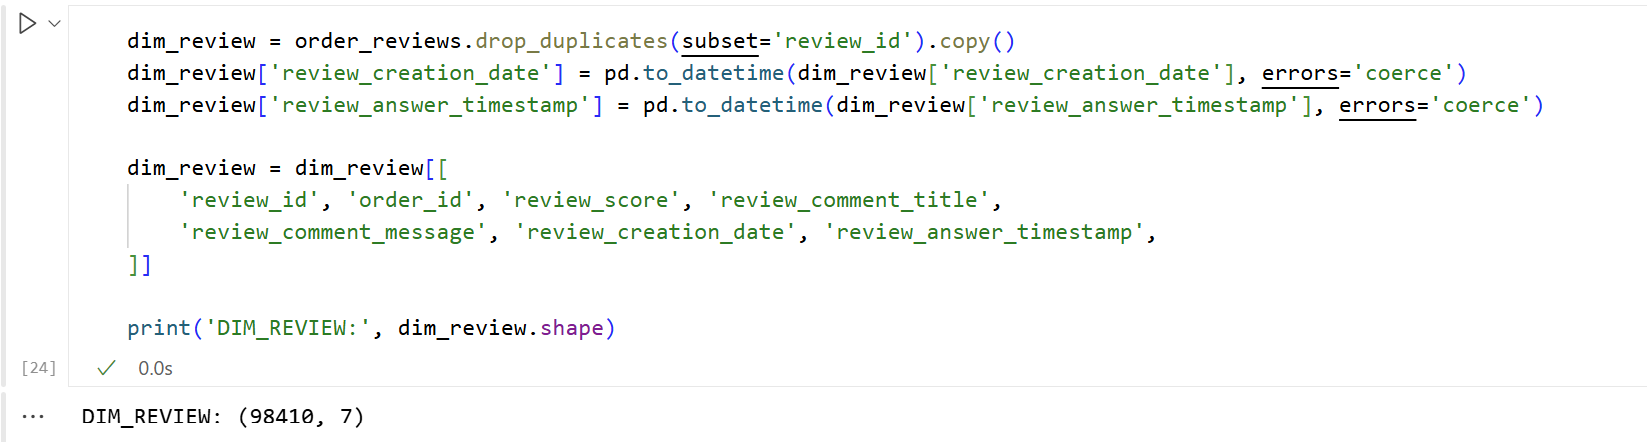
\includegraphics[width=\textwidth]{img_c1/c1_fig21_dim_review.png}
    \caption{Cấu trúc hoàn thiện của bảng chiều đánh giá \texttt{DIM\_REVIEW}}
    \label{fig:c1f21}
\end{figure}

{\footnotesize
\begin{longtable}{@{}p{4.7cm}p{2.1cm}p{8.2cm}@{}}
\caption{Các thuộc tính của bảng \texttt{DIM\_REVIEW}}\label{tab:dimreview}\\
\toprule
\textbf{Tên thuộc tính} & \textbf{Kiểu dữ liệu} & \textbf{Ý nghĩa}\\
\midrule
\endfirsthead
\multicolumn{3}{@{}l}{\textit{Bảng \ref{tab:dimreview} (tiếp theo)}}\\
\toprule
\textbf{Tên thuộc tính} & \textbf{Kiểu dữ liệu} & \textbf{Ý nghĩa}\\
\midrule
\endhead
\midrule
\multicolumn{3}{r@{}}{\textit{(xem tiếp trang sau)}}\\
\endfoot
\bottomrule
\endlastfoot
\texttt{review\_id} & string & Mã phiếu đánh giá, khóa chính\\
\texttt{order\_id} & string & Mã đơn hàng (khóa ngoại tới \texttt{FACT\_ORDER\_ITEMS})\\
\texttt{review\_score} & integer & Điểm đánh giá của khách, từ 1 đến 5\\
\texttt{review\_comment\_title} & string & Tiêu đề nhận xét do khách nhập\\
\texttt{review\_comment\_message} & string & Nội dung nhận xét do khách nhập\\
\texttt{review\_creation\_date} & datetime & Ngày phiếu khảo sát được gửi tới khách hàng\\
\texttt{review\_answer\_timestamp} & datetime & Thời điểm khách hàng trả lời khảo sát\\
\end{longtable}}

\subsubsection{Xây dựng và mô tả chi tiết các bảng Sự kiện (Fact Tables)}

Sau khi toàn bộ các bảng chiều đã hoàn thiện và sẵn sàng làm từ điển tra cứu, ba bảng sự kiện (Fact) được khởi tạo theo các mức độ chi tiết (grain) và nghiệp vụ đo lường riêng biệt.

\paragraph{Bảng sự kiện chi tiết đơn hàng (FACT\_ORDER\_ITEMS)}

Bảng sự kiện trung tâm \texttt{FACT\_ORDER\_ITEMS} có grain ở mức chi tiết nhất (atomic grain): mỗi dòng biểu diễn một sản phẩm trong đơn hàng, xác định bởi khóa chính kết hợp \texttt{(order\_id, order\_item\_id)}. Bảng được tạo bằng cách nối bảng chi tiết mặt hàng (\texttt{order\_items}) với bảng đơn hàng (\texttt{orders}) để bổ sung khóa ngoại \texttt{customer\_id}, đồng thời liên kết tới \texttt{DIM\_SELLER} và \texttt{DIM\_PRODUCT}. Bảng lưu trữ hai độ đo tài chính cốt lõi: đơn giá (\texttt{price}) và cước phí vận chuyển (\texttt{freight\_value}), với tổng quy mô 112.650 bản ghi.

\begin{figure}[H]
    \centering
    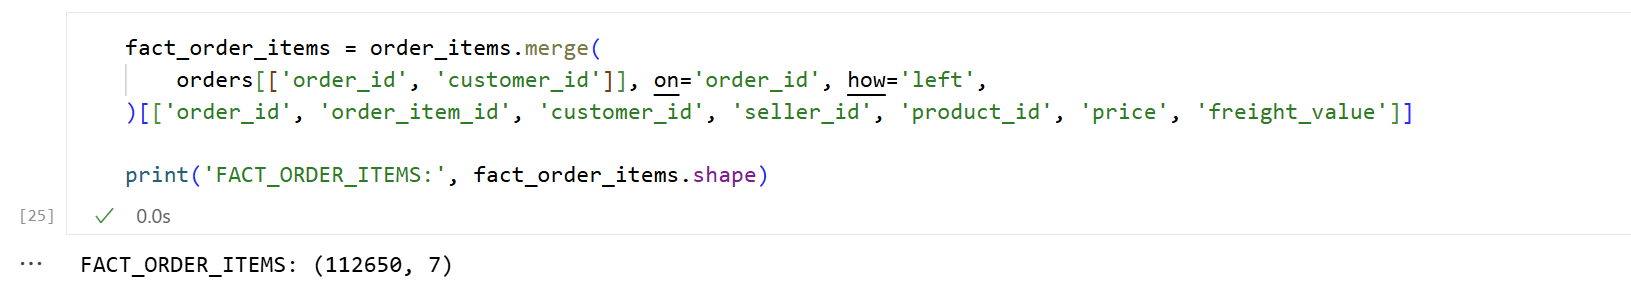
\includegraphics[width=\textwidth]{img_c1/c1_fig22_fact_order_items.png}
    \caption{Xây dựng bảng sự kiện chi tiết đơn hàng \texttt{FACT\_ORDER\_ITEMS}}
    \label{fig:c1f22}
\end{figure}

{\footnotesize
\begin{longtable}{@{}p{4.7cm}p{2.1cm}p{8.2cm}@{}}
\caption{Các thuộc tính của bảng \texttt{FACT\_ORDER\_ITEMS}}\label{tab:factorderitems}\\
\toprule
\textbf{Tên thuộc tính} & \textbf{Kiểu dữ liệu} & \textbf{Ý nghĩa}\\
\midrule
\endfirsthead
\multicolumn{3}{@{}l}{\textit{Bảng \ref{tab:factorderitems} (tiếp theo)}}\\
\toprule
\textbf{Tên thuộc tính} & \textbf{Kiểu dữ liệu} & \textbf{Ý nghĩa}\\
\midrule
\endhead
\midrule
\multicolumn{3}{r@{}}{\textit{(xem tiếp trang sau)}}\\
\endfoot
\bottomrule
\endlastfoot
\texttt{order\_id} & string & Mã đơn hàng, khóa chính cùng với \texttt{order\_item\_id}\\
\texttt{order\_item\_id} & integer & Số thứ tự của sản phẩm trong cùng một đơn hàng\\
\texttt{customer\_id} & string & Mã khách hàng gắn với từng đơn hàng, khóa chính (khóa ngoại tới \texttt{DIM\_CUSTOMER})\\
\texttt{seller\_id} & string & Mã người bán, khóa chính (khóa ngoại tới \texttt{DIM\_SELLER})\\
\texttt{product\_id} & string & Mã sản phẩm, khóa chính (khóa ngoại tới \texttt{DIM\_PRODUCT})\\
\texttt{price} & float & Giá bán của sản phẩm, đơn vị Real Brazil (BRL)\\
\texttt{freight\_value} & float & Phí vận chuyển phân bổ cho dòng sản phẩm này (BRL)\\
\end{longtable}}

\paragraph{Bảng sự kiện thanh toán (FACT\_ORDER\_PAYMENT)}

Bảng sự kiện thanh toán \texttt{FACT\_ORDER\_PAYMENT} có grain ở mức từng giao dịch thanh toán, xác định bởi cặp khóa \texttt{(order\_id, payment\_sequential)}. Bảng được tách riêng khỏi bảng chi tiết mặt hàng do khác biệt về mức độ chi tiết (một đơn hàng có thể có nhiều đợt hoặc nhiều phương thức thanh toán khác nhau). Thiết kế này giúp theo dõi chính xác dòng tiền thanh toán (\texttt{payment\_value}) và số kỳ trả góp (\texttt{payment\_installments}) mà không gây dư thừa hay nhân bản doanh thu đơn hàng.

\begin{figure}[H]
    \centering
    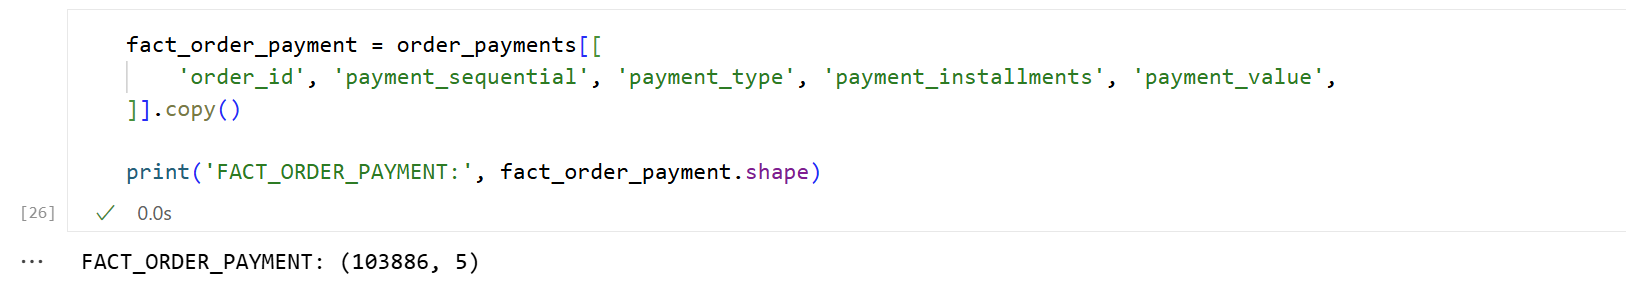
\includegraphics[width=\textwidth]{img_c1/c1_fig23_fact_order_payment.png}
    \caption{Xây dựng bảng sự kiện thanh toán \texttt{FACT\_ORDER\_PAYMENT}}
    \label{fig:c1f23}
\end{figure}

{\footnotesize
\begin{longtable}{@{}p{4.7cm}p{2.1cm}p{8.2cm}@{}}
\caption{Các thuộc tính của bảng \texttt{FACT\_ORDER\_PAYMENT}}\label{tab:factorderpayment}\\
\toprule
\textbf{Tên thuộc tính} & \textbf{Kiểu dữ liệu} & \textbf{Ý nghĩa}\\
\midrule
\endfirsthead
\multicolumn{3}{@{}l}{\textit{Bảng \ref{tab:factorderpayment} (tiếp theo)}}\\
\toprule
\textbf{Tên thuộc tính} & \textbf{Kiểu dữ liệu} & \textbf{Ý nghĩa}\\
\midrule
\endhead
\midrule
\multicolumn{3}{r@{}}{\textit{(xem tiếp trang sau)}}\\
\endfoot
\bottomrule
\endlastfoot
\texttt{order\_id} & string & Mã đơn hàng (khóa ngoại tới \texttt{FACT\_ORDER\_ITEMS})\\
\texttt{payment\_sequential} & integer & Số thứ tự của lần thanh toán trong cùng một đơn hàng\\
\texttt{payment\_type} & string & Hình thức thanh toán\\
\texttt{payment\_installments} & integer & Số kỳ trả góp của lần thanh toán\\
\texttt{payment\_value} & float & Số tiền của lần thanh toán (BRL)\\
\end{longtable}}

\paragraph{Bảng sự kiện khách hàng tiềm năng (FACT\_SELLER\_LEAD)}

Bảng sự kiện phễu tiếp thị \texttt{FACT\_SELLER\_LEAD} theo dõi quá trình chuyển đổi đối tác kinh doanh: mỗi dòng tương ứng với một khách hàng tiềm năng (lead), xác định bởi khóa chính \texttt{mql\_id}. Bảng được xây dựng bằng phép \texttt{LEFT JOIN} từ 8.000 leads đủ điều kiện (\texttt{leads\_qualified}) sang bảng chốt hợp đồng (\texttt{leads\_closed}) theo \texttt{mql\_id}. Cờ nhị phân \texttt{is\_won} được tạo để phân biệt lead đã chốt hợp đồng thành công thành người bán (\texttt{seller\_id}). Các trường dữ liệu tự khai (doanh thu kỳ vọng, phân khúc, quy mô kho bãi...) được giữ nguyên để phục vụ phân tích hiệu quả phễu chuyển đổi.

\begin{figure}[H]
    \centering
    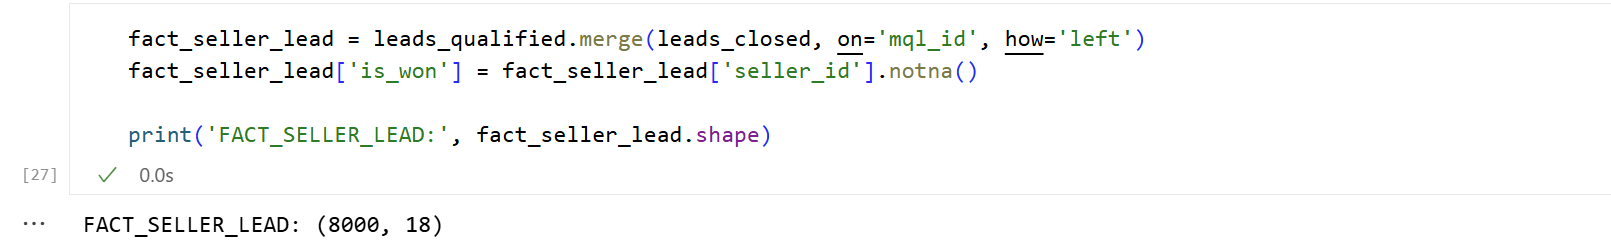
\includegraphics[width=\textwidth]{img_c1/c1_fig24_fact_seller_lead.png}
    \caption{Xây dựng bảng sự kiện phễu tiếp thị \texttt{FACT\_SELLER\_LEAD}}
    \label{fig:c1f24}
\end{figure}

{\footnotesize
\begin{longtable}{@{}p{4.7cm}p{2.1cm}p{8.2cm}@{}}
\caption{Các thuộc tính của bảng \texttt{FACT\_SELLER\_LEAD}}\label{tab:factsellerlead}\\
\toprule
\textbf{Tên thuộc tính} & \textbf{Kiểu dữ liệu} & \textbf{Ý nghĩa}\\
\midrule
\endfirsthead
\multicolumn{3}{@{}l}{\textit{Bảng \ref{tab:factsellerlead} (tiếp theo)}}\\
\toprule
\textbf{Tên thuộc tính} & \textbf{Kiểu dữ liệu} & \textbf{Ý nghĩa}\\
\midrule
\endhead
\midrule
\multicolumn{3}{r@{}}{\textit{(xem tiếp trang sau)}}\\
\endfoot
\bottomrule
\endlastfoot
\texttt{mql\_id} & string & Mã khách hàng tiềm năng đã qua sàng lọc, khóa chính\\
\texttt{first\_contact\_date} & string & Ngày lead điền biểu mẫu liên hệ lần đầu\\
\texttt{landing\_page\_id} & string & Mã trang đích mà lead truy cập\\
\texttt{origin} & string & Kênh đưa lead đến sàn\\
\texttt{seller\_id} & string & Mã người bán, khóa chính (khóa ngoại tới \texttt{DIM\_SELLER})\\
\texttt{sdr\_id} & string & Mã nhân viên phát triển kinh doanh tiếp nhận lead\\
\texttt{sr\_id} & string & Mã nhân viên bán hàng chốt hợp đồng\\
\texttt{won\_date} & string & Thời điểm lead chính thức trở thành người bán\\
\texttt{business\_segment} & string & Phân khúc ngành hàng của người bán\\
\texttt{lead\_type} & string & Loại hình lead\\
\texttt{lead\_behaviour\_profile} & string & Hồ sơ hành vi của lead\\
\texttt{has\_company} & float & Lead đã có pháp nhân đăng ký hay chưa\\
\texttt{has\_gtin} & float & Sản phẩm của lead đã có mã vạch GTIN hay chưa\\
\texttt{average\_stock} & string & Khoảng tồn kho trung bình do lead tự khai\\
\texttt{business\_type} & string & Loại hình kinh doanh\\
\texttt{declared\_product\_catalog\_size} & float & Số lượng sản phẩm trong danh mục do lead tự khai\\
\texttt{declared\_monthly\_revenue} & float & Doanh thu hằng tháng do lead tự khai (BRL)\\
\texttt{is\_won} & boolean & Cờ đánh dấu lead đã chuyển đổi thành người bán\\
\end{longtable}}

\subsubsection{Kiểm tra tính toàn vẹn tham chiếu}

Sau khi hoàn thiện các bảng Fact và Dim, tính toàn vẹn tham chiếu khóa ngoại (Foreign Key Integrity) giữa các bảng sự kiện và bảng chiều trên lược đồ đích được kiểm tra tự động bằng mã kiểm thử (Hình~\ref{fig:c1f25}).

\begin{figure}[H]
    \centering
    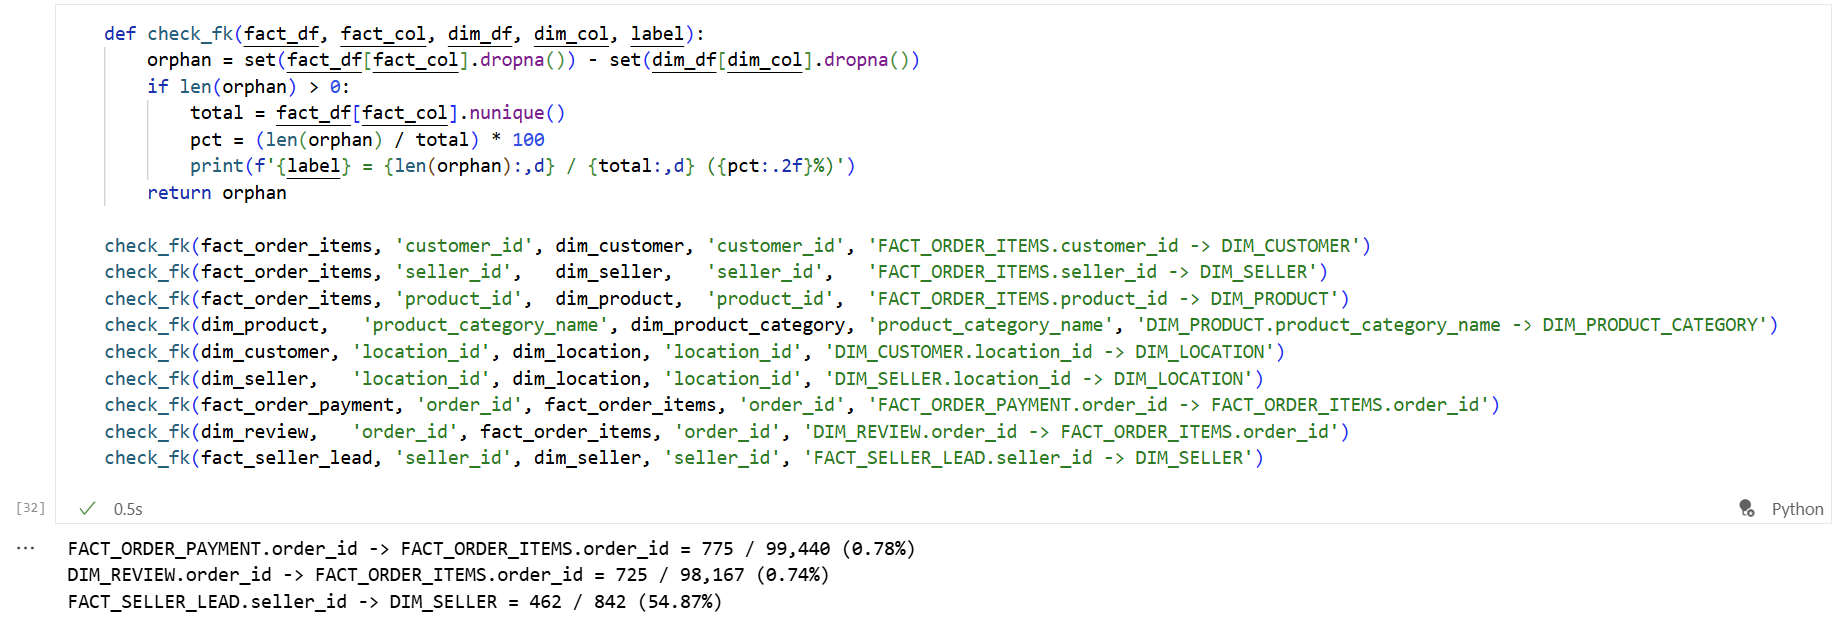
\includegraphics[width=\textwidth]{img_c1/c1_fig25_kiem_tra_referential_integrity_schema.png}
    \caption{Kiểm tra tính toàn vẹn tham chiếu giữa các bảng sự kiện và bảng chiều}
    \label{fig:c1f25}
\end{figure}

Kết quả kiểm tra xác nhận phần lớn các khóa ngoại liên kết tới các bảng chiều khách hàng, người bán, sản phẩm và địa điểm đều đạt tính toàn vẹn tuyệt đối 100\% (0 bản ghi orphan). Ba mối quan hệ ghi nhận bản ghi orphan được giải thích thỏa đáng theo đặc thù nghiệp vụ như sau:
\begin{enumerate}\setlength{\itemsep}{2pt}
  \item \textbf{\texttt{FACT\_ORDER\_PAYMENT.order\_id} $\to$ \texttt{FACT\_ORDER\_ITEMS.order\_id} (775 orphan / 99.440 đơn, 0.78\%):} Khách hàng đã thanh toán thành công qua cổng thanh toán, nhưng đơn hàng sau đó bị hủy (\texttt{canceled}) hoặc không có hàng giao (\texttt{unavailable}) trước khi chi tiết sản phẩm được ghi nhận trong kho. Đây là hiện tượng nghiệp vụ thực tế của dòng tiền, không phải lỗi ETL. Dữ liệu này được giữ nguyên nhằm phục vụ bài toán đối soát tài chính và hoàn tiền.
  \item \textbf{\texttt{DIM\_REVIEW.order\_id} $\to$ \texttt{FACT\_ORDER\_ITEMS.order\_id} (725 orphan / 98.167 đơn, 0.74\%):} Tương tự trường hợp thanh toán, khách hàng gửi đánh giá trải nghiệm cho các đơn hàng đã bị hủy hoặc sự cố trước khi xử lý mặt hàng.
  \item \textbf{\texttt{FACT\_SELLER\_LEAD.seller\_id} $\to$ \texttt{DIM\_SELLER.seller\_id} (462 orphan / 842 đối tác, 54.87\%):} Như đã phân tích chi tiết tại mục~\ref{subsec:tienxuly}, 462 đối tác đã ký hợp đồng thành công nhưng chưa từng phát sinh đơn hàng nào trên sàn, do đó chưa xuất hiện trong danh mục người bán vận hành.
\end{enumerate}

% --------------------------------------------------
